\documentclass[11pt]{article}

\usepackage[margin=1in]{geometry}
\usepackage{booktabs}
\usepackage{tabularx}
\usepackage{hyperref}
\usepackage{parskip}
\usepackage{amsmath}
\usepackage{amssymb}
\usepackage{extarrows}
\usepackage{tikz}
\usetikzlibrary{positioning, arrows.meta, calc, decorations.pathreplacing, fit, backgrounds}

\setlength{\emergencystretch}{1em}

\hypersetup{
  colorlinks=true,
  linkcolor=blue,
  urlcolor=blue,
  citecolor=blue
}

\title{Real-Time Web Communication Standards:\\A Retrospective and Projection\\2021--2031}
\author{}
\date{March 2026}

\begin{document}
\maketitle

\tableofcontents
\listoffigures
\listoftables
\newpage

\section{Introduction}

This document examines the concrete browser capabilities enabled by the
real-time web communication standards collected in the \texttt{standards/}
directory of this project. It compares what these standards made possible in
browsers as of late 2021 with what they enable as of March 2026. The
discussion focuses exclusively on what standards adoption in browsers enabled
--- not on market trends, product adoption, or commercial developments.

The standards under review span five areas:
\begin{itemize}
  \item \textbf{WebRTC} --- W3C WebRTC 1.0 and supporting IETF protocols
    (RFCs 8829, 8445, 8826, 8827, 3550, 3711)
  \item \textbf{QUIC} --- RFC 9000
  \item \textbf{HTTP/3} --- RFC 9114
  \item \textbf{WebTransport} --- W3C Working Draft and RFC 9297
  \item \textbf{WebCodecs} --- W3C Working Draft
\end{itemize}

Together, these standards define a full stack for real-time communication in
the browser: from low-level transport (QUIC) through application-layer
protocols (HTTP/3, WebTransport) to peer-to-peer media and data exchange
(WebRTC) and direct codec access (WebCodecs).

\section{WebRTC}

The WebRTC stack in the \texttt{standards/} directory comprises the W3C
WebRTC 1.0 specification and six IETF RFCs: JSEP (RFC~8829), ICE
(RFC~8445), the WebRTC security considerations (RFC~8826), the DTLS-based
security architecture (RFC~8827), RTP (RFC~3550), and SRTP (RFC~3711).

\subsection{Late 2021}

W3C WebRTC 1.0 achieved Recommendation status in January 2021, making it a
finalized standard. By late 2021, Chrome and Firefox offered full
implementations, and Edge inherited Chrome's support via its Chromium base.
Safari supported the core API but with significant limitations:

\begin{itemize}
  \item \textbf{Codec restrictions.} Safari supported only H.264 for video.
    Chrome and Firefox supported VP8, VP9, and H.264. This meant Safari could
    not participate in VP9-based calls and lacked access to VP9's more
    efficient bandwidth usage.
  \item \textbf{No simulcast or SVC.} Safari could not send multiple
    encodings of the same video stream at different resolutions (simulcast)
    or use Scalable Video Coding (SVC). Chrome and Firefox supported both,
    enabling adaptive quality based on network conditions.
  \item \textbf{RTCDataChannel issues on iOS.} The data channel did not work
    reliably on iOS Safari. Cross-browser data channel connections between
    Safari on iOS and Chrome or Firefox failed due to missing local ICE
    candidates on iOS.
  \item \textbf{SDP handling divergence.} Chrome was in the process of
    migrating from Plan~B to Unified Plan SDP semantics. Chrome~M89
    (February 2021) added deprecation warnings; Chrome~M93 (August 2021)
    removed Plan~B with a reverse origin trial option. Firefox and Safari
    already used Unified Plan exclusively. During this transition, applications
    had to accommodate both SDP formats.
  \item \textbf{Insertable Streams.} Chrome~M94 introduced the
    Insertable Streams API, enabling JavaScript to access and transform
    encoded media frames in the WebRTC pipeline. This was essential for
    end-to-end encryption of media. Firefox and Safari did not implement it.
  \item \textbf{Stats reporting inconsistencies.} Firefox was missing
    \texttt{voice\-Activity\-Flag} on video track stats. Safari was missing
    \texttt{rtpTimestamp} and \texttt{voiceActivityFlag}. Applications could
    not reliably detect voice activity or obtain precise timing information
    across browsers.
\end{itemize}

On the IETF side, the supporting protocols were in the following state:
\begin{itemize}
  \item \textbf{JSEP (RFC~8829)} was published in January 2021 alongside the
    W3C Recommendation. All browsers implemented the JSEP signaling
    state machine through \texttt{RTCPeerConnection}, but diverged in areas
    like BUNDLE handling of multiple media streams.
  \item \textbf{ICE (RFC~8445)} was implemented in all browsers. Trickle ICE
    (RFC~8838), enabling incremental candidate exchange rather than waiting for
    full gathering, was published in January 2021 but not yet mandatory.
  \item \textbf{DTLS-SRTP (RFCs~8827, 3711)} was mandatory across all
    browsers. All media was encrypted. However, browsers differed in DTLS
    certificate algorithms (Chrome~52+ used ECDSA; others varied), and
    privacy identifier reset mechanisms were inconsistent.
  \item \textbf{Security (RFC~8826)} --- all browsers enforced
    camera/microphone permission prompts and encrypted all media. However,
    protections against IP address leakage were inconsistent; not all browsers
    masked local IP addresses via mDNS candidates when media permissions had
    not been granted.
\end{itemize}

\subsection{March 2026}

The W3C updated the WebRTC 1.0 Recommendation in October 2024 and again in
2025, incorporating amendments based on implementation experience.

\begin{itemize}
  \item \textbf{Unified Plan is universal.} Plan~B SDP is completely removed
    from all browsers. Applications no longer need to accommodate both formats.
  \item \textbf{Safari gained VP9.} Safari~15 and later support the VP9 codec
    for WebRTC, enabling Safari to participate in VP9-based calls and benefit
    from VP9's bandwidth efficiency. Safari still prefers H.264 for hardware
    acceleration, and its SVC support remains limited compared to
    Chrome and Firefox.
  \item \textbf{iOS WebRTC matured.} Starting with iOS~14.3, WebRTC works
    reliably across all browsers on iOS. RTCDataChannel connections between
    iOS Safari and desktop Chrome or Firefox are reliable.
  \item \textbf{JSEP updated to RFC~9429.} Published in April 2024, RFC~9429
    obsoleted RFC~8829, addressing implementation divergence --- particularly
    in BUNDLE handling and bundle-only \texttt{m=} sections.
  \item \textbf{Trickle ICE is mandatory.} All browsers implement RFC~8838,
    enabling faster connection establishment through incremental candidate
    exchange.
  \item \textbf{mDNS privacy protections standardized.} Chrome, Firefox, and
    Safari all mask local IP addresses using mDNS candidates when
    camera/microphone permissions have not been granted, implementing the
    privacy considerations of RFC~8826.
  \item \textbf{Encoded Transforms remain Chrome-only.} The feature
    evolved from ``Insertable Streams'' to \texttt{RTCRtp\-Script\-Transform}
    (WebRTC Encoded Transform), but Firefox and Safari still do not
    implement it. End-to-end encryption of encoded media frames in the
    WebRTC pipeline remains a Chrome/Chromium-only capability.
\end{itemize}

\section{QUIC}

RFC~9000 defines the QUIC transport protocol: a UDP-based, multiplexed,
encrypted transport with built-in TLS~1.3, independent stream flow control,
and connection migration across network changes.

\subsection{Late 2021}

RFC~9000 was published in May 2021. Browser support was uneven:

\begin{itemize}
  \item \textbf{Chrome} had QUIC enabled by default, having been an early
    adopter (Google developed the original QUIC protocol).
  \item \textbf{Firefox~88} (April 2021) enabled QUIC by default.
  \item \textbf{Safari} had experimental QUIC support (added in Safari
    Technology Preview~104, April 2020), but it required manual opt-in
    through experimental settings. It was not available to ordinary users.
\end{itemize}

In practice, a browser connecting to a QUIC-capable server would benefit from
reduced connection latency (0-RTT or 1-RTT handshakes vs.\ TCP's multi-round
handshake plus TLS), elimination of head-of-line blocking across multiplexed
streams, and connection survival across network changes. But with Safari
requiring manual opt-in, these benefits were unavailable to most Safari users.

\subsection{March 2026}

QUIC is enabled by default in all major browsers:
\begin{itemize}
  \item Chrome, Edge, and Firefox continue default support.
  \item Safari~16 (2022) enabled QUIC by default, bringing universal coverage.
\end{itemize}

Every major browser can now establish QUIC connections transparently. The
capabilities defined by RFC~9000 --- low-latency connection establishment,
multiplexed streams without head-of-line blocking, built-in encryption, and
connection migration --- are universally available to web applications without
any user or developer opt-in.

\section{HTTP/3}

RFC~9114 maps HTTP semantics over QUIC, inheriting QUIC's transport
properties: multiplexed streams without head-of-line blocking, lower
connection latency, and connection migration.

\subsection{Late 2021}

RFC~9114 had not yet been published (it was finalized in June 2022). Browsers
were shipping pre-standard HTTP/3 implementations based on draft
specifications:

\begin{itemize}
  \item \textbf{Chrome} had experimental HTTP/3 support enabled by default
    since April 2020.
  \item \textbf{Firefox~88} (April 2021) enabled HTTP/3 by default.
  \item \textbf{Safari} had HTTP/3 support behind an experimental feature
    flag, disabled by default.
\end{itemize}

Where supported, browsers could negotiate HTTP/3 with compatible servers,
gaining per-stream independence (a stalled stream would not block other
streams, unlike HTTP/2 over TCP). However, the lack of a finalized RFC meant
implementations were based on draft specifications that could diverge, and
Safari's experimental-only status limited universal availability.

\subsection{March 2026}

With RFC~9114 finalized in June 2022, all major browsers now support HTTP/3
by default:
\begin{itemize}
  \item Chrome, Edge, and Firefox have supported HTTP/3 by default for
    several years.
  \item Safari enabled HTTP/3 by default starting with Safari~16 (2022).
  \item Over 92\% of browser market share supports HTTP/3.
\end{itemize}

The capabilities defined by RFC~9114 --- HTTP request/response multiplexing
without head-of-line blocking, lower latency connection establishment via
QUIC, and connection resilience across network changes --- are now universally
available. Any browser connecting to an HTTP/3-capable server automatically
benefits from these properties.

\section{WebTransport}

The WebTransport specification defines browser APIs for bidirectional
client-server communication over HTTP/3, supporting both reliable streams and
unreliable datagrams. RFC~9297 defines the HTTP datagram and capsule protocol
mechanisms that underpin it.

\subsection{Late 2021}

WebTransport was in a very early state:

\begin{itemize}
  \item \textbf{Chrome} had experimental support but it was disabled in
    Chrome~M91 through M94. The API was not usable in production.
  \item \textbf{Firefox} had no support whatsoever.
  \item \textbf{Safari} had no support whatsoever.
  \item RFC~9297 had not yet been published (August 2022).
  \item The W3C specification was an early Working Draft.
\end{itemize}

In late 2021, WebTransport was effectively unavailable in any browser for
production use. The capabilities it defines --- unreliable datagrams from
browser to server, multiple independent reliable streams, and connection
migration --- could not be used by web applications.

\subsection{March 2026}

WebTransport has achieved broad but not universal support:

\begin{itemize}
  \item \textbf{Chrome~97+} and \textbf{Edge~98+} support WebTransport
    (stable since late 2021 / early 2022).
  \item \textbf{Firefox~114+} (2023) supports WebTransport.
  \item \textbf{Safari does not support WebTransport.}
  \item Approximately 82\% of browser market share has WebTransport support.
\end{itemize}

For browsers that support it, WebTransport enables capabilities that were
previously impossible without WebRTC's peer-to-peer architecture:
\begin{itemize}
  \item \textbf{Unreliable datagrams} from browser to server, suitable for
    latency-sensitive data where retransmission is undesirable (e.g., game
    state updates, real-time sensor data).
  \item \textbf{Multiple independent reliable streams} without head-of-line
    blocking between them, enabling parallel data flows over a single
    connection.
  \item \textbf{Connection migration} across network changes, inherited from
    QUIC.
\end{itemize}

Safari's absence means applications using WebTransport must provide fallback
mechanisms (typically WebSocket) for Safari users, or accept that these
capabilities are unavailable on Apple platforms.

\section{WebCodecs}

The WebCodecs specification provides JavaScript interfaces for direct access
to the browser's built-in audio, video, and image codecs, enabling
frame-level encoding and decoding outside of higher-level APIs like
\texttt{MediaRecorder} or \texttt{HTMLMediaElement}.

\subsection{Late 2021}

WebCodecs had just reached initial availability:

\begin{itemize}
  \item \textbf{Chrome~94} (September 2021) shipped WebCodecs as a stable
    feature, graduating from origin trial. Chrome~92 and 93 had offered it
    as an origin trial with breaking changes between versions.
  \item \textbf{Firefox} had no support.
  \item \textbf{Safari} had no support.
  \item The W3C specification was a First Public Working Draft (2021).
\end{itemize}

In Chrome~94, developers could for the first time:
\begin{itemize}
  \item Encode and decode individual video frames using
    \texttt{VideoEncoder} and \texttt{VideoDecoder} with the browser's
    hardware-accelerated codecs, without being constrained by
    \texttt{MediaRecorder}'s real-time recording model.
  \item Encode and decode individual audio chunks
    (\texttt{AudioEncoder}/\texttt{AudioDecoder}).
  \item Perform faster-than-realtime encoding (previously impossible via
    \texttt{MediaRecorder}).
  \item Control per-frame keyframe insertion and quality parameters.
  \item Obtain raw encoded bytes without container overhead.
\end{itemize}

However, these capabilities were Chrome-only. Firefox and Safari users had no
access to low-level codec APIs; they were limited to the high-level
\texttt{MediaRecorder} and \texttt{HTMLMediaElement} interfaces.

\subsection{March 2026}

WebCodecs has achieved broad cross-browser support:

\begin{itemize}
  \item \textbf{Chrome/Edge} --- supported since version 94 (2021).
  \item \textbf{Firefox~130+} (September 2024) --- shipped approximately three
    years after Chrome.
  \item \textbf{Safari~26+} (2024) --- full support. Earlier Safari versions
    (16.4+) had partial video-only support.
  \item Approximately 94\% of browser market share supports WebCodecs.
  \item The specification remains a W3C Working Draft (updated January 2026),
    not yet a Recommendation.
\end{itemize}

With cross-browser support, all major browsers can now perform frame-level
codec operations using hardware acceleration. This enables web applications
to build custom media pipelines --- video editors, live transcoders, custom
streaming clients --- that were previously possible only through WebAssembly
codec implementations or native applications.

\section{Summary}

\begin{table}[ht]
\centering
\small
\renewcommand{\arraystretch}{1.3}
\begin{tabularx}{\textwidth}{lXXX}
\toprule
\textbf{Standard} & \textbf{Late 2021} & \textbf{March 2026} & \textbf{Key Change} \\
\midrule
WebRTC 1.0 &
  W3C Rec (Jan 2021). Chrome/Firefox full support. Safari limited: H.264 only, no simulcast, iOS DataChannel broken. Plan~B still in Chrome. &
  Updated Rec (2024--25). Unified Plan universal. Safari has VP9. iOS reliable. JSEP updated to RFC~9429. mDNS privacy standardized. &
  Uneven $\to$ converged (Safari gap narrowed; Encoded Transforms still Chrome-only) \\
\midrule
QUIC &
  RFC~9000 (May 2021). Chrome/Firefox default. Safari experimental, manual opt-in. &
  Default in all browsers (Safari~16+, 2022). &
  Partial $\to$ universal \\
\midrule
HTTP/3 &
  Pre-RFC draft implementations. Chrome/Firefox default. Safari behind flag. &
  RFC~9114 (June 2022). Default in all browsers. 92\%+ coverage. &
  Draft $\to$ standard $\to$ universal \\
\midrule
WebTransport &
  Experimental only. Chrome disabled (M91--94). Firefox/Safari: none. &
  Chrome~97+, Firefox~114+. Safari: still absent. 82\% coverage. &
  Non-functional $\to$ broadly available (Safari gap) \\
\midrule
WebCodecs &
  Chrome~94 only (Sept 2021). Firefox/Safari: none. First Public WD. &
  Chrome, Firefox~130+, Safari~26+. 94\% coverage. Still WD. &
  Chrome-only $\to$ cross-browser \\
\bottomrule
\end{tabularx}
\caption{Browser capability status by standard, late 2021 vs.\ March 2026.}
\label{tab:summary}
\end{table}

\section{Conclusion}

In late 2021, the real-time web communication stack defined by these standards
was in a transitional state. WebRTC was the only finalized standard with
broad browser support, yet even it suffered from significant cross-browser
inconsistencies --- Safari's codec and feature limitations, Chrome's ongoing
SDP migration, and iOS reliability issues. QUIC had just been standardized
but was not yet universally enabled. HTTP/3 was shipping in browsers based on
draft specifications, without a finalized RFC. WebTransport was effectively
non-functional in any browser. WebCodecs had just shipped in a single
browser.

By March 2026, the picture is fundamentally different. The entire protocol
stack --- from QUIC transport through HTTP/3 to WebRTC --- is standardized
via finalized RFCs and implemented by default across all major browsers.
WebCodecs provides cross-browser access to hardware-accelerated codecs at the
frame level. The most notable remaining gap is Safari's lack of WebTransport
support, which prevents universal availability of browser-to-server unreliable
datagrams and independent reliable streams. The Encoded Transforms API for
WebRTC also remains Chrome-only, limiting cross-browser end-to-end encryption
of media in the WebRTC pipeline.

The practical consequence is that a web application built in March 2026 can
rely on a complete, standards-based real-time communication stack across all
major browsers --- something that was not possible in late 2021, when much of
the stack was either draft, experimental, single-browser, or absent.

\section{Looking Ahead: 2028--2029 (Two to Three Years)}

The following projections are grounded in active W3C charter milestones, IETF
draft publication timelines, and formal browser vendor implementation signals.

\subsection{WebCodecs Reaches W3C Recommendation}

The W3C Media Working Group charter targets WebCodecs Candidate
Recommendation in Q1~2026 and full Recommendation by Q4~2026. By 2028, the
specification should be a mature, finalized standard. This means the
frame-level codec access that was Chrome-only in 2021 and cross-browser by
2026 will have a stable, locked-down API surface that browser vendors commit
to maintaining long-term. The WebCodecs Codec Registry will likely include
formal AV1 registration entries alongside existing H.264, VP8, and VP9
entries.

\subsection{WebTransport Achieves Universal Browser Support}

Apple committed WebTransport as a formal Interop~2026 priority, accounting
for 20\% of the interoperability score. Safari already has experimental
WebTransport support behind a flag in iOS~18. Given this commitment, Safari
production support is expected by late 2026 or early 2027, with the W3C
specification reaching Recommendation status around the same time. By 2028,
WebTransport should be universally available across all major browsers ---
closing the last significant gap in the stack. Applications will be able to
rely on browser-to-server unreliable datagrams and independent reliable
streams without Safari fallbacks.

\subsection{WebRTC Encoded Transforms Become Cross-Browser}

The \texttt{RTCRtpScriptTransform} API (WebRTC Encoded Transform) has a
Working Draft dated February 2026 and is approaching Candidate
Recommendation. Safari and Firefox have implemented it natively; Chrome
continues support via its earlier Insertable Streams lineage. By 2028, this
API should be standardized and available across all major browsers, enabling
cross-browser end-to-end encryption of media frames within the WebRTC
pipeline --- a capability that was Chrome-only from 2021 through 2026.

\subsection{AV1 Becomes a Practical WebRTC Codec}

Firefox enabled AV1 for WebRTC by default in 2025. Chrome has supported it
for several years. By 2028, AV1 hardware encoding support in consumer devices
will have expanded, reducing the CPU cost that currently limits its adoption.
AV1's superior compression efficiency (roughly 30\% better than VP9 at
equivalent quality) will make it a practical default codec for WebRTC calls
in Chrome and Firefox. Safari's adoption remains uncertain, as Apple
historically favors H.264 with hardware acceleration.

\subsection{Media over QUIC Reaches RFC Status}

The IETF Media over QUIC (MoQ) transport draft
(\texttt{draft-ietf-moq-transport}) is advancing rapidly, with version~15
published in October 2025. The protocol enables subscription-based media
publishing and consuming over QUIC, designed for low-latency distribution
with CDN support. By 2028, MoQ should have reached RFC status, along with
companion specifications for media container formats (Low Overhead Media
Container) and streaming formats. Browser integration will likely occur
through JavaScript libraries built on WebTransport and WebCodecs rather than
through dedicated browser APIs --- the component APIs are already in place to
support this.

\subsection{RTP over QUIC Reaches RFC Status}

The IETF RTP over QUIC (RoQ) draft (\texttt{draft-ietf-avtcore-rtp-over-quic})
maps RTP and RTCP packets onto QUIC streams and datagrams. By 2028, this
should reach RFC status, enabling WebRTC backends to transport media over
QUIC instead of the traditional UDP+DTLS-SRTP path. Browser-facing
integration would occur through SDP negotiation rather than new JavaScript
APIs, potentially enabling WebRTC calls to benefit from QUIC's congestion
control and connection migration at the transport layer.

\subsection{Hardware and Network Context}

The standards projections above do not exist in a vacuum. By 2028, two
underlying trends amplify what these standards make practically possible.

\textbf{CPU and hardware acceleration.} AV1 encoding is computationally
expensive --- in 2026, real-time AV1 encoding for a WebRTC call can consume
an entire CPU core on mid-range hardware, which is why VP9 and H.264 remain
the practical defaults despite AV1's superior compression. By 2028, dedicated
AV1 hardware encoders will be standard in new laptops, phones, and tablets
(Apple's M-series chips, Qualcomm Snapdragon, Intel Arc, and AMD RDNA
already include or are adding AV1 encode blocks). This shifts AV1 from
``technically supported but too expensive'' to ``hardware-accelerated and
free.'' The WebCodecs API, which exposes hardware-accelerated codecs to
JavaScript, directly benefits: an application calling
\texttt{VideoEncoder} with AV1 in 2028 will hit dedicated silicon rather than
a software encoder, making frame-level AV1 processing via WebCodecs
practical for real-time use cases.

Similarly, the unbundled architecture --- composing WebTransport, WebCodecs,
and WebAssembly --- imposes CPU overhead from JavaScript orchestration and
WebAssembly processing that would have been prohibitive on 2021 hardware.
By 2028, the roughly 40--50\% improvement in single-thread CPU performance
since 2021 (compounding at approximately 8--10\% annually) makes this
overhead manageable for real-time media pipelines.

\textbf{Network bandwidth.} Global median fixed broadband speeds have
approximately doubled from 2021 to 2026 (from roughly 60~Mbps to over
120~Mbps in developed markets), and 5G mobile networks have expanded
substantially. By 2028, continued growth in fixed and mobile bandwidth
means that the efficiency gains from AV1 and QUIC compound with raw
bandwidth increases. A WebRTC call using AV1 over QUIC on a 2028 connection
will have both a more efficient codec (30\% less bandwidth than VP9) and
more available bandwidth, enabling higher resolution and frame rates within
the same network cost envelope. QUIC's connection migration (RFC~9000)
becomes more impactful as mobile usage grows --- a video call that seamlessly
survives a Wi-Fi to 5G handoff requires both the protocol support (already
standardized) and sufficient mobile bandwidth to sustain the call (increasingly
available).

The net effect is that the standards reaching maturity by 2028 will land on
hardware and networks that can fully exploit them, rather than being
bottlenecked by the infrastructure they run on.

\begin{figure}[ht]
\centering
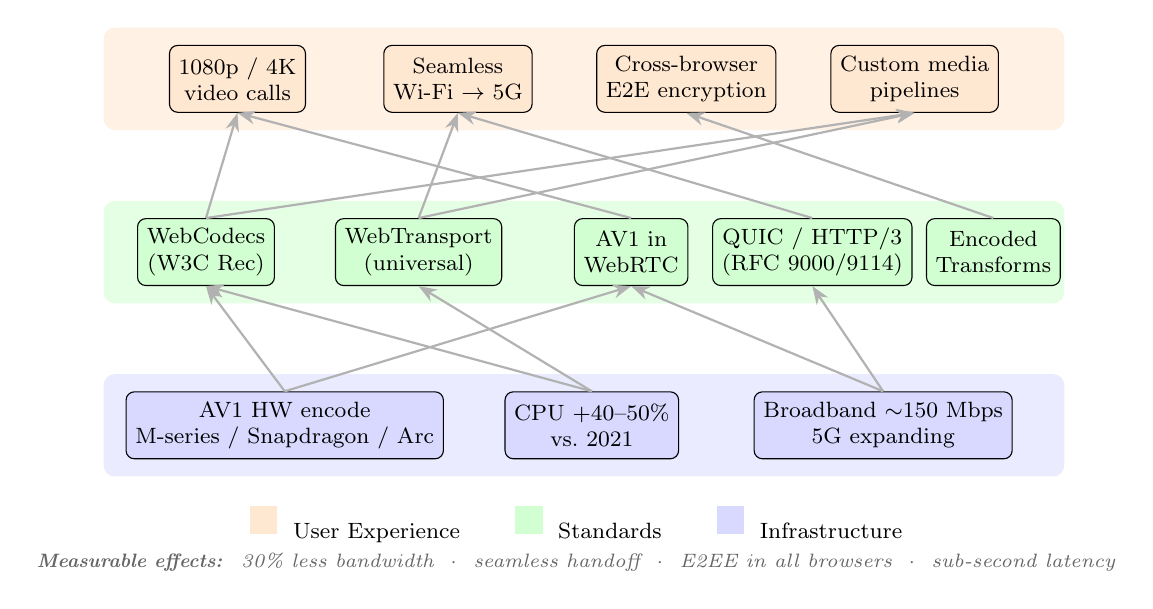
\begin{tikzpicture}[
  >=Stealth,
  item/.style={draw, rounded corners=3pt, minimum height=0.85cm,
    align=center, font=\footnotesize, fill=white},
  arr/.style={->, thick, gray!60},
  metriclabel/.style={font=\scriptsize\itshape, text=black!60},
]

% --- Layer background bands (no border, distinct colors) ---
\fill[blue!8, rounded corners=4pt]
  (-5.5, -0.65) rectangle (6.7, 0.65);
\fill[green!10, rounded corners=4pt]
  (-5.5, 1.55) rectangle (6.7, 2.85);
\fill[orange!10, rounded corners=4pt]
  (-5.5, 3.75) rectangle (6.7, 5.05);

% --- Infrastructure items ---
\node[item, fill=blue!15] (hw) at (-3.2, 0)
  {AV1 HW encode\\M-series / Snapdragon / Arc};
\node[item, fill=blue!15] (cpu) at (0.7, 0)
  {CPU +40--50\%\\vs.\ 2021};
\node[item, fill=blue!15] (net) at (4.4, 0)
  {Broadband ${\sim}$150~Mbps\\5G expanding};

% --- Standards items ---
\node[item, fill=green!18] (wc) at (-4.2, 2.2)
  {WebCodecs\\(W3C Rec)};
\node[item, fill=green!18] (wt) at (-1.5, 2.2)
  {WebTransport\\(universal)};
\node[item, fill=green!18] (av1) at (1.2, 2.2)
  {AV1 in\\WebRTC};
\node[item, fill=green!18] (quic) at (3.5, 2.2)
  {QUIC / HTTP/3\\(RFC 9000/9114)};
\node[item, fill=green!18] (et) at (5.8, 2.2)
  {Encoded\\Transforms};

% --- User experience items ---
\node[item, fill=orange!18] (hd) at (-3.8, 4.4)
  {1080p / 4K\\video calls};
\node[item, fill=orange!18] (handoff) at (-1.0, 4.4)
  {Seamless\\Wi-Fi $\to$ 5G};
\node[item, fill=orange!18] (e2ee) at (1.9, 4.4)
  {Cross-browser\\E2E encryption};
\node[item, fill=orange!18] (custom) at (4.8, 4.4)
  {Custom media\\pipelines};

% --- Arrows: infrastructure -> standards ---
\draw[arr] (hw.north) -- (wc.south);
\draw[arr] (hw.north) -- (av1.south);
\draw[arr] (cpu.north) -- (wt.south);
\draw[arr] (cpu.north) -- (wc.south);
\draw[arr] (net.north) -- (quic.south);
\draw[arr] (net.north) -- (av1.south);

% --- Arrows: standards -> user experience ---
\draw[arr] (wc.north) -- (hd.south);
\draw[arr] (wc.north) -- (custom.south);
\draw[arr] (av1.north) -- (hd.south);
\draw[arr] (wt.north) -- (custom.south);
\draw[arr] (wt.north) -- (handoff.south);
\draw[arr] (quic.north) -- (handoff.south);
\draw[arr] (et.north) -- (e2ee.south);

% --- Legend (below diagram, horizontal) ---
\node[anchor=north, font=\footnotesize] at (0.5, -0.9) {%
  \tikz[baseline=-0.5ex]{\fill[orange!18] (0,0) rectangle (0.35,0.35);}
  ~User Experience \qquad
  \tikz[baseline=-0.5ex]{\fill[green!18] (0,0) rectangle (0.35,0.35);}
  ~Standards \qquad
  \tikz[baseline=-0.5ex]{\fill[blue!15] (0,0) rectangle (0.35,0.35);}
  ~Infrastructure};

% --- Measurable effects ---
\node[metriclabel, anchor=north, align=center] at (0.5, -1.5)
  {\textbf{Measurable effects:} ~30\% less bandwidth
   ~$\cdot$~ seamless handoff ~$\cdot$~
   E2EE in all browsers ~$\cdot$~ sub-second latency};

\end{tikzpicture}
\caption{By 2028: infrastructure enables standards to deliver measurable
  user experience gains. Arrows show enabling relationships.}
\label{fig:2028-stack}
\end{figure}

\section{Looking Ahead: 2029--2031 (Three to Five Years)}

These projections extend further from current standardization activity and
carry correspondingly more uncertainty, but follow from the trajectory
established by the standards work described above.

\subsection{The ``Unbundled'' Architecture Becomes Viable}

By 2029, all the component APIs --- WebTransport (universal), WebCodecs
(Recommendation), and RTCRtpScriptTransform (standardized) --- will have been
stable and cross-browser for two or more years. This makes the ``WebRTC
Unbundled'' architecture practically viable: applications can compose
WebTransport for data transport, WebCodecs for encoding and decoding, and
WebAssembly for custom processing, bypassing the monolithic
\texttt{RTCPeerConnection} API entirely.

This matters because the unbundled approach gives applications control over
decisions that WebRTC currently makes internally: which codec to use, how to
packetize, what transport to use, and how to handle congestion. Use cases
that are poorly served by WebRTC's built-in assumptions --- cloud gaming
requiring ultra-low latency with acceptable loss, scientific visualization
requiring custom frame processing, or broadcast distribution requiring
one-to-many fan-out --- can be built from these composable primitives.

Traditional WebRTC via \texttt{RTCPeerConnection} will persist for general
video conferencing, where its built-in codec negotiation, ICE connectivity,
and DTLS-SRTP security provide a well-integrated default. The unbundled
approach is not a replacement but an alternative for applications with
specialized requirements.

\begin{figure}[ht]
\centering
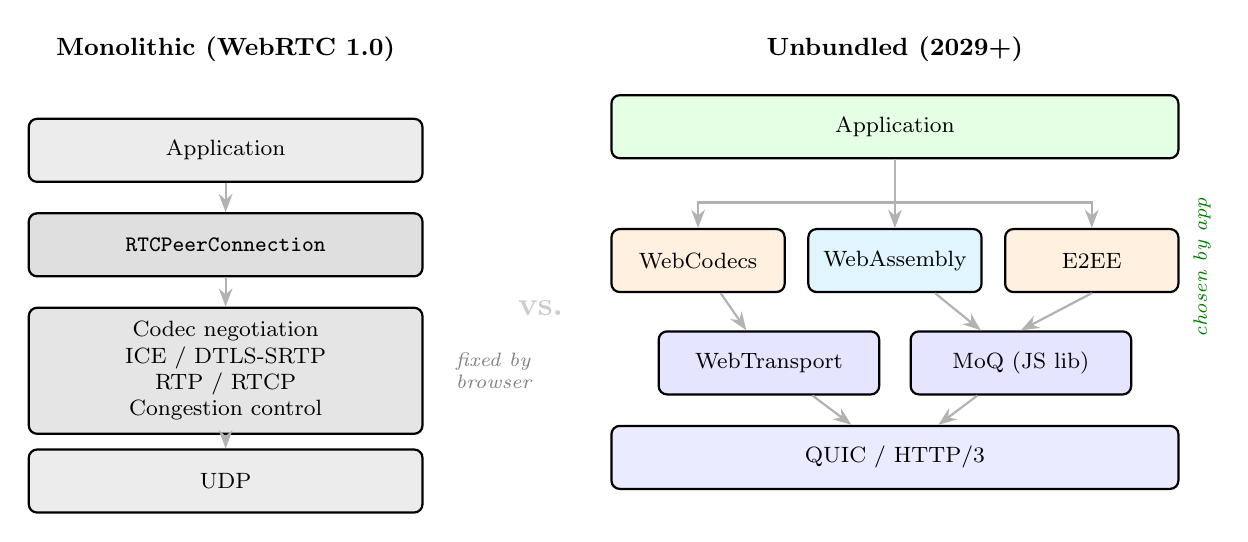
\begin{tikzpicture}[
  >=Stealth,
  block/.style={draw, rounded corners=3pt, minimum height=0.8cm,
    align=center, font=\footnotesize, thick},
  monolith/.style={block, fill=gray!15, minimum width=5cm},
  unbundled/.style={block, fill=green!10, minimum width=2.6cm},
  label/.style={font=\small\bfseries, anchor=south},
  arr/.style={->, thick, gray!60},
  brace/.style={decorate, decoration={brace, amplitude=6pt, mirror}},
]

% --- Monolithic side (left) ---
\node[label] at (-3.5, 5.5) {Monolithic (WebRTC 1.0)};

\node[monolith] (app1) at (-3.5, 4.5) {Application};
\node[monolith, fill=gray!25] (rtc) at (-3.5, 3.3) {\texttt{RTCPeerConnection}};
\node[monolith, fill=gray!20, minimum height=1.6cm] (internals) at (-3.5, 1.7)
  {Codec negotiation\\ICE / DTLS-SRTP\\RTP / RTCP\\Congestion control};
\node[monolith] (udp1) at (-3.5, 0.3) {UDP};

\draw[arr] (app1) -- (rtc);
\draw[arr] (rtc) -- (internals);
\draw[arr] (internals) -- (udp1);

% fixed / chosen by browser label
\node[font=\scriptsize\itshape, text=gray, anchor=west] at (-0.7, 1.7) {\parbox{1.1cm}{fixed by\\browser}};

% --- Unbundled side (right) ---
\node[label] at (5.0, 5.5) {Unbundled (2029+)};

\node[unbundled, minimum width=7.2cm] (app2) at (5.0, 4.8) {Application};

\node[unbundled, fill=orange!12, minimum width=2.2cm] (wcodec) at (2.5, 3.1) {WebCodecs};
\node[unbundled, fill=cyan!12, minimum width=2.2cm] (wasm) at (5.0, 3.1) {WebAssembly};
\node[unbundled, fill=orange!12, minimum width=2.2cm] (et2) at (7.5, 3.1) {E2EE};

\node[unbundled, fill=blue!10, minimum width=2.8cm] (wtrans) at (3.4, 1.8) {WebTransport};
\node[unbundled, fill=blue!10, minimum width=2.8cm] (moq) at (6.6, 1.8) {MoQ (JS lib)};

\node[unbundled, fill=blue!8, minimum width=7.2cm] (quicl) at (5.0, 0.6) {QUIC / HTTP/3};

\draw[arr] (app2.south) -- ++(0,-0.55) -| (wcodec.north);
\draw[arr] (app2.south) -- ++(0,-0.55) -| (wasm.north);
\draw[arr] (app2.south) -- ++(0,-0.55) -| (et2.north);
\draw[arr] (wcodec) -- (wtrans);
\draw[arr] (wasm) -- (moq);
\draw[arr] (et2.south) -- (moq.north);
\draw[arr] (wtrans) -- (quicl);
\draw[arr] (moq) -- (quicl);

% chosen by application label
\node[font=\scriptsize\itshape, text=green!50!black, anchor=west,
  rotate=90] at (8.9, 2.0) {chosen by app};

% --- "vs" divider ---
\node[font=\large\bfseries, text=gray!40] at (0.5, 2.5) {vs.};

\end{tikzpicture}
\caption{Monolithic WebRTC (left) vs.\ the unbundled architecture (right).
  The unbundled approach gives applications control over codec, transport,
  encryption, and congestion decisions that \texttt{RTCPeerConnection}
  handles internally.}
\label{fig:unbundled}
\end{figure}

\subsection{MoQ Enables Standards-Based Low-Latency Streaming}

With MoQ at RFC status and WebTransport universally available, a
standards-based path exists for low-latency media streaming from server to
browser that does not require WebRTC. A MoQ JavaScript library running on
WebTransport and using WebCodecs for decoding could deliver sub-second
latency streaming with CDN fan-out --- combining the latency characteristics
previously unique to WebRTC with the scalability of traditional CDN
architectures. This creates a standards-based alternative to proprietary
low-latency streaming protocols.

\subsection{AV1 as the Default WebRTC Codec}

By 2030, hardware AV1 encoding will be standard in consumer devices
(laptops, phones, tablets). The CPU cost barrier that limits AV1 adoption in
2026 will have largely disappeared. AV1's compression advantage over VP9 and
H.264 makes it the natural default for WebRTC, reducing bandwidth
requirements for equivalent video quality. Whether Safari adopts AV1 for
WebRTC depends on Apple's hardware acceleration decisions, but the broader
ecosystem pressure from Chrome and Firefox --- which together represent the
majority of browser usage --- will make AV1 the dominant codec for new
WebRTC applications.

\subsection{QUIC v2 Transparent Adoption}

QUIC~v2 (RFC~9369, published May 2023) is identical to QUIC~v1 in capability
but uses different wire constants to resist middlebox ossification. By 2030,
browsers will have transparently migrated to QUIC~v2 for new connections.
This is invisible to applications --- no new capabilities are exposed --- but
ensures the QUIC transport layer remains resilient against network
intermediaries that might otherwise interfere with the protocol based on
recognizing v1 byte patterns.

\subsection{No WebRTC 2.0}

The W3C WebRTC Working Group charter (extending to September 2026) adds new
capabilities through extension specifications rather than monolithic version
bumps. This pattern is expected to continue. There will be no ``WebRTC~2.0''
in the traditional sense. Instead, the API surface will grow incrementally
through standardized extensions --- Encoded Transforms, SFrame for
end-to-end encryption in group calls, and future extensions not yet drafted
--- while the core \texttt{RTCPeerConnection} API remains stable.

\subsection{Hardware and Network Context}

By 2030, the hardware and network landscape further amplifies the practical
impact of these matured standards.

\textbf{CPU and hardware acceleration.} By 2030, single-thread CPU
performance will have improved roughly 60--80\% relative to 2021 levels,
and AV1 hardware encode/decode will be ubiquitous --- present not just in
flagship devices but in budget laptops and mid-range phones. This has two
consequences for the standards discussed here. First, AV1 becomes the
natural default codec for WebRTC: the hardware acceleration eliminates the
CPU cost barrier, and WebCodecs applications calling \texttt{VideoEncoder}
with AV1 will consistently hit dedicated silicon across the device spectrum,
not just on high-end hardware. Second, the unbundled architecture ---
WebTransport plus WebCodecs plus WebAssembly --- becomes practical even on
resource-constrained devices. The JavaScript and WebAssembly orchestration
overhead that would strain a 2021 mobile processor is routine on a 2030
device, making custom real-time media pipelines viable on phones and tablets,
not just desktop machines.

\textbf{Network bandwidth.} If current trends hold, median fixed broadband
speeds in developed markets will reach 200--300~Mbps by 2030, with 5G mobile
networks providing reliable 100+~Mbps in urban areas. At these speeds,
bandwidth is no longer the binding constraint for most real-time
communication scenarios. The practical consequence is a shift in what
matters: codec efficiency (AV1 over H.264) becomes less about fitting within
tight bandwidth limits and more about enabling higher quality --- 4K video
conferencing, high-frame-rate screen sharing, or multi-stream layouts ---
without saturating the connection. QUIC's multiplexed streams (RFC~9000)
and HTTP/3's head-of-line blocking elimination (RFC~9114) matter most when
multiple parallel flows compete for bandwidth, which is precisely the
scenario enabled by abundant bandwidth and ambitious applications.

MoQ-based streaming benefits particularly from this environment. A MoQ
library on WebTransport using WebCodecs to decode AV1 can deliver
high-bitrate, low-latency streams that would have been impractical in 2021
not because the standards didn't exist, but because the combination of codec
cost, network capacity, and API availability wasn't there. By 2030, all
three constraints are resolved simultaneously: the standards are finalized
and universal, the hardware accelerates the codecs, and the networks carry
the bits.

\textbf{The compounding effect.} The key observation is that standards
maturation, hardware improvement, and network growth are complementary, not
independent. A standard that reaches browser universality on hardware that
can't run it efficiently, or over networks that can't carry its output,
delivers theoretical capability rather than practical impact. By the
2029--2031 timeframe, these three curves converge: every standard in this
document will be finalized and universally implemented, running on hardware
with dedicated acceleration for the codecs they specify, over networks with
bandwidth to spare. This convergence is what makes the 3--5 year outlook
qualitatively different from a simple extrapolation of today's capabilities.

\begin{figure}[ht]
\centering
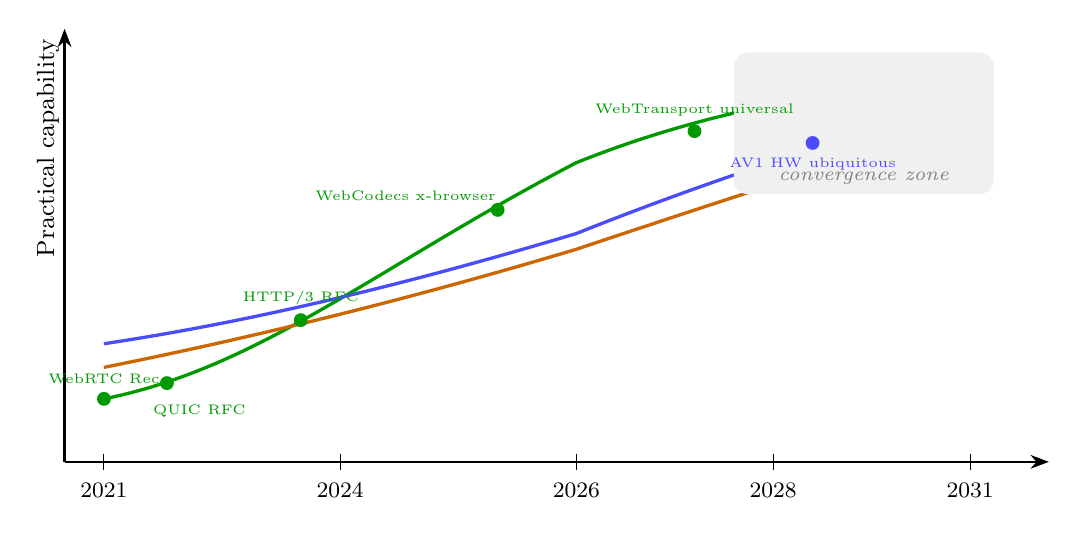
\begin{tikzpicture}[
  >=Stealth,
]

% --- Axes ---
\draw[->, thick] (0, 0) -- (12.5, 0) node[anchor=north, font=\small] {};
\draw[->, thick] (0, 0) -- (0, 5.5) node[anchor=east, font=\small, rotate=90,
  yshift=6pt] {Practical capability};

% Year labels
\foreach \x/\yr in {0.5/2021, 3.5/2024, 6.5/2026, 9/2028, 11.5/2031} {
  \draw (\x, -0.1) -- (\x, 0.1);
  \node[font=\footnotesize, anchor=north] at (\x, -0.15) {\yr};
}

% --- Standards maturity curve (green) ---
\draw[very thick, green!60!black]
  (0.5, 0.8) .. controls (2.5, 1.2) and (4, 2.5) ..
  (6.5, 3.8) .. controls (8, 4.4) and (9.5, 4.7) ..
  (11.5, 4.9);
\node[font=\scriptsize, green!60!black, anchor=south west] at (10.2, 4.85)
  {Standards};

% --- Hardware capability curve (blue) ---
\draw[very thick, blue!70]
  (0.5, 1.5) .. controls (2.5, 1.8) and (4.5, 2.3) ..
  (6.5, 2.9) .. controls (8, 3.5) and (9.5, 4.0) ..
  (11.5, 4.6);
\node[font=\scriptsize, blue!70, anchor=south west] at (10.2, 4.4)
  {Hardware};

% --- Network bandwidth curve (orange) ---
\draw[very thick, orange!80!black]
  (0.5, 1.2) .. controls (2.5, 1.6) and (4.5, 2.1) ..
  (6.5, 2.7) .. controls (8, 3.2) and (9.5, 3.7) ..
  (11.5, 4.3);
\node[font=\scriptsize, orange!80!black, anchor=south west] at (10.2, 3.95)
  {Network};

% --- Convergence zone ---
\fill[gray!12, rounded corners=5pt] (8.5, 3.4) rectangle (11.8, 5.2);
\node[font=\scriptsize\itshape, text=black!50, align=center] at (10.15, 3.6)
  {convergence zone};

% --- Key milestones (annotation dots) ---
% WebRTC 1.0 Rec
\fill[green!60!black] (0.5, 0.8) circle (2.5pt);
\node[font=\tiny, anchor=south, green!60!black, yshift=2pt] at (0.5, 0.8)
  {WebRTC Rec};

% QUIC RFC
\fill[green!60!black] (1.3, 1.0) circle (2.5pt);
\node[font=\tiny, anchor=north west, green!60!black] at (1.0, 0.85)
  {QUIC RFC};

% HTTP/3 RFC
\fill[green!60!black] (3.0, 1.8) circle (2.5pt);
\node[font=\tiny, anchor=south, green!60!black, yshift=2pt] at (3.0, 1.8)
  {HTTP/3 RFC};

% WebCodecs cross-browser
\fill[green!60!black] (5.5, 3.2) circle (2.5pt);
\node[font=\tiny, anchor=south east, green!60!black] at (5.6, 3.2)
  {WebCodecs x-browser};

% WebTransport universal (projected)
\fill[green!60!black] (8.0, 4.2) circle (2.5pt);
\node[font=\tiny, anchor=south, green!60!black, yshift=2pt] at (8.0, 4.2)
  {WebTransport universal};

% AV1 HW ubiquitous
\fill[blue!70] (9.5, 4.05) circle (2.5pt);
\node[font=\tiny, anchor=north, blue!70, yshift=-2pt] at (9.5, 4.05)
  {AV1 HW ubiquitous};

\end{tikzpicture}
\caption{Convergence of standards maturity, hardware capability, and network
  bandwidth from 2021 to 2031. The shaded region marks where all three curves
  reach levels sufficient to fully exploit the standards discussed in this
  document.}
\label{fig:convergence}
\end{figure}

\appendix
% appendix-info-theory.tex
% Standalone appendix — include from retrospective.tex via:
%   \appendix
%   % appendix-info-theory.tex
% Standalone appendix — include from retrospective.tex via:
%   \appendix
%   % appendix-info-theory.tex
% Standalone appendix — include from retrospective.tex via:
%   \appendix
%   \input{appendix-info-theory}
%
% Requires in the preamble: amsmath, amssymb, tabularx, booktabs

\section{Information-Theoretic View}
\label{app:info-theory}

This appendix applies information-theoretic measures to the real-time
web communication stack described in this document. We quantify channel
capacity, source coding efficiency, and effective information rates
across three time horizons: today (March~2026), the near term
(2027--2028), and the medium term (2029--2031). The analysis draws on
the standards, codec parameters, and infrastructure projections
developed in the main text.

\subsection{Channel Capacity of the Transport Layer}

The Shannon-Hartley theorem gives the theoretical maximum information
rate for a channel with additive white Gaussian noise:
\begin{equation}
  C = B \log_2\!\left(1 + \frac{S}{N}\right) \quad \text{[bits/s]}
  \label{eq:shannon}
\end{equation}
where $B$ is the channel bandwidth in Hz and $S/N$ is the
signal-to-noise ratio.

While the physical-layer capacity of a broadband link is governed by
(\ref{eq:shannon}), the \emph{effective} capacity available to the
application is reduced by protocol overhead, congestion control, and
transport inefficiencies. We define the effective application-layer
throughput as:
\begin{equation}
  R_{\text{eff}} = C_{\text{link}} \cdot \eta_{\text{transport}}
    \cdot (1 - \rho_{\text{overhead}})
  \label{eq:reff}
\end{equation}
where $C_{\text{link}}$ is the link-layer capacity,
$\eta_{\text{transport}} \in (0,1]$ is the transport efficiency factor
(capturing congestion control, retransmission, and multiplexing
behavior), and $\rho_{\text{overhead}} \in [0,1)$ is the fractional
protocol overhead (headers, encryption, framing).

\subsubsection{Head-of-Line Blocking and Multiplexed Capacity}

Consider $n$ independent streams multiplexed over a single connection.
Under TCP (HTTP/2), a single lost packet blocks all $n$ streams. The
expected throughput per stream under loss rate $p$ is bounded by:
\begin{equation}
  R_{\text{TCP}}^{(i)} \leq \frac{R_{\text{eff}}}{n}
    \cdot (1 - p)^{n-1}
  \label{eq:hol-tcp}
\end{equation}
because a loss in \emph{any} of the $n$ streams stalls all others. Under
QUIC (RFC~9000), streams are independent at the transport layer, so:
\begin{equation}
  R_{\text{QUIC}}^{(i)} \leq \frac{R_{\text{eff}}}{n}
    \cdot (1 - p)
  \label{eq:hol-quic}
\end{equation}
The ratio of effective per-stream throughput is:
\begin{equation}
  \frac{R_{\text{QUIC}}^{(i)}}{R_{\text{TCP}}^{(i)}}
    = \frac{1}{(1-p)^{n-2}}
  \label{eq:hol-ratio}
\end{equation}
\excursus{Excursus: Why $n = 8$?}{In a typical multi-participant video
conference, each peer contributes multiple concurrent streams: a camera video
track, an audio track, and often a screen-share or data channel. A four-person
call with two media tracks each produces $n = 8$ multiplexed streams over a
single connection --- the reference value used throughout this section. Larger
meetings (e.g.\ 10 participants with simulcast layers) push $n$ higher,
amplifying the HOL blocking effect further.}

For $n = 8$ streams (a typical multi-track video conference) at
$p = 0.01$ (1\% loss), this gives a QUIC advantage factor of
$1/(0.99)^6 \approx 1.062$, a modest 6.2\% improvement. At $p = 0.05$
(5\% loss, common on mobile or congested links), the factor is
$1/(0.95)^6 \approx 1.34$, a 34\% throughput advantage per stream.

\begin{figure}[ht]
\centering
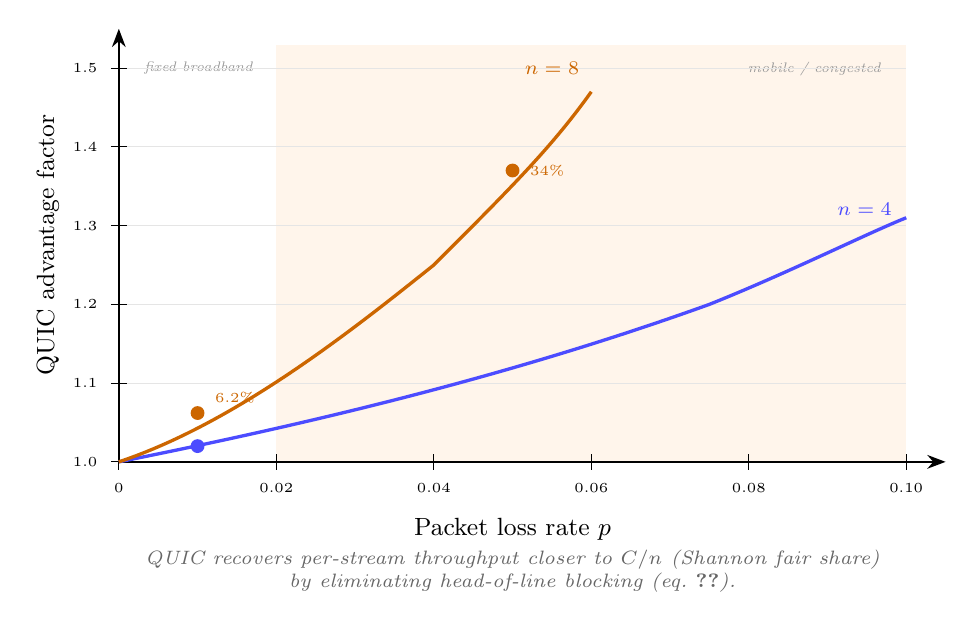
\begin{tikzpicture}[>=Stealth]

% --- Shaded region (drawn FIRST so curves appear on top) ---
\fill[orange!8] (2, 0) rectangle (10, 5.3);
\node[font=\tiny\itshape, text=black!40, anchor=north east] at (9.8, 5.2)
  {mobile / congested};
\node[font=\tiny\itshape, text=black!40, anchor=north west] at (0.2, 5.2)
  {fixed broadband};

% --- Grid lines ---
\foreach \y in {1, 2, 3, 4, 5} {
  \draw[gray!20] (0, \y) -- (10, \y);
}

% --- Axes ---
\draw[->, thick] (0, 0) -- (10.5, 0);
\draw[->, thick] (0, 0) -- (0, 5.5);

% --- Axis titles (positioned to clear tick labels) ---
\node[font=\small] at (5, -0.85) {Packet loss rate $p$};
\node[font=\small, rotate=90] at (-0.9, 2.75) {QUIC advantage factor};

% --- X-axis labels ---
\foreach \x/\lab in {0/0, 2/0.02, 4/0.04, 6/0.06, 8/0.08, 10/0.10} {
  \draw (\x, -0.1) -- (\x, 0.1);
  \node[font=\tiny, anchor=north] at (\x, -0.15) {\lab};
}

% --- Y-axis labels ---
\foreach \y/\lab in {0/1.0, 1/1.1, 2/1.2, 3/1.3, 4/1.4, 5/1.5} {
  \draw (-0.1, \y) -- (0.1, \y);
  \node[font=\tiny, anchor=east] at (-0.15, \y) {\lab};
}

% --- n=4 curve: 1/(1-p)^2 ---
\draw[very thick, blue!70]
  (0, 0) .. controls (2.5, 0.5) and (5, 1.1) ..
  (7.5, 2.0) .. controls (8.5, 2.4) and (9.5, 2.9) ..
  (10, 3.1);
\node[font=\scriptsize, blue!70, anchor=south west] at (9.0, 3.0)
  {$n = 4$};

% --- n=8 curve: 1/(1-p)^6 ---
\draw[very thick, orange!80!black]
  (0, 0) .. controls (1.5, 0.5) and (3, 1.7) ..
  (4, 2.5) .. controls (5, 3.5) and (5.5, 4.0) ..
  (6, 4.7);
\node[font=\scriptsize, orange!80!black, anchor=south] at (5.5, 4.8)
  {$n = 8$};

% --- Reference points ---
\fill[orange!80!black] (1.0, 0.62) circle (2.5pt);
\node[font=\tiny, orange!80!black, anchor=south west] at (1.1, 0.62)
  {6.2\%};

\fill[orange!80!black] (5.0, 3.7) circle (2.5pt);
\node[font=\tiny, orange!80!black, anchor=west] at (5.1, 3.7)
  {34\%};

\fill[blue!70] (1.0, 0.20) circle (2.5pt);

% --- Annotation ---
\node[font=\scriptsize\itshape, text=black!60, align=center,
  anchor=north] at (5.0, -1.0)
  {QUIC recovers per-stream throughput closer to $C/n$ (Shannon fair share)\\
   by eliminating head-of-line blocking (eq.~\ref{eq:hol-ratio}).};

\end{tikzpicture}
\caption{QUIC advantage factor $1/(1-p)^{n-2}$ over TCP for multiplexed
  streams. At 5\% loss with $n=8$ streams, QUIC delivers 34\% more
  per-stream throughput by maintaining independence at the transport layer.}
\label{fig:hol-blocking}
\end{figure}

\subsubsection{Connection Establishment Latency}

Let $\tau$ denote the one-way latency (half the round-trip time). The
information-carrying capacity during connection establishment is zero;
the handshake represents pure overhead. The time to first useful byte
is:
\begin{align}
  T_{\text{TCP+TLS\,1.3}} &= 2\tau_{\text{TCP}} + \tau_{\text{TLS}}
    = 3\tau \quad \text{(1-RTT TLS~1.3)} \label{eq:tcp-setup} \\
  T_{\text{QUIC}} &= \tau \quad \text{(1-RTT)}
    \label{eq:quic-setup} \\
  T_{\text{QUIC,\,0-RTT}} &= 0 \quad \text{(resumption)}
    \label{eq:quic-0rtt}
\end{align}
The QUIC 0-RTT case (\ref{eq:quic-0rtt}) eliminates the handshake
entirely for resumed connections. The information lost during
handshake dead time, relative to steady-state capacity, is:
\begin{equation}
  I_{\text{lost}} = C_{\text{link}} \cdot T_{\text{setup}}
  \label{eq:ilost}
\end{equation}
For a 120~Mbps link with $\tau = 25$~ms (typical fixed broadband in
2026), the TCP+TLS~1.3 handshake wastes $120 \times 10^6 \times 0.075
= 9 \times 10^6$ bits (1.125~MB), while QUIC~1-RTT wastes only
$3 \times 10^6$ bits (375~KB).

\subsection{Source Coding Efficiency}

The rate-distortion function $R(D)$ defines the minimum bit rate
required to represent a source at distortion level $D$. For a
Gaussian source with variance $\sigma^2$ under mean squared error
distortion:
\begin{equation}
  R(D) = \frac{1}{2} \log_2 \frac{\sigma^2}{D}
    \quad \text{[bits/sample]}
  \label{eq:rate-distortion}
\end{equation}

\excursus{Excursus: Why Gaussian source?}{The Gaussian memoryless model is used
because it yields the highest (worst-case) $R(D)$ among all sources of equal
variance. Any codec that approaches the Gaussian bound on real video is
therefore doing at least as well as the bound predicts --- the true $R(D)$ for
spatially and temporally correlated video lies below the Gaussian curve, making
it a conservative benchmark.}

No practical codec achieves $R(D)$;\footnote{The $R(D)$ curve in
Figure~\ref{fig:rate-distortion} is the Gaussian memoryless source bound
(equation~\ref{eq:rate-distortion}), which is an upper bound on the true
$R(D)$ for non-Gaussian sources such as video.  Additionally, $R(D)$ assumes
zero excess-distortion probability, whereas practical codecs permit a
frame-level excess-distortion probability on the order of $10^{-6}$ to
$10^{-8}$.  Both factors allow codec operating points measured on real content
to approach or marginally cross the Gaussian bound.} real codecs operate at
some rate $R_{\text{codec}} > R(D)$. We define the coding efficiency gap as:
\begin{equation}
  \Delta = \frac{R_{\text{codec}} - R(D)}{R(D)}
  \label{eq:coding-gap}
\end{equation}

The codecs in the WebRTC stack can be ordered by their empirical
proximity to $R(D)$ for typical video content at conversational
resolutions (720p, 30~fps). Using published Bj\o ntegaard Delta (BD)
rate measurements:
\begin{equation}
  R_{\text{H.264}} > R_{\text{VP9}} > R_{\text{AV1}}
    > R(D)
  \label{eq:codec-ordering}
\end{equation}

Specifically, the empirical rate savings at equivalent PSNR are
approximately:
\begin{align}
  R_{\text{VP9}}  &\approx 0.65 \cdot R_{\text{H.264}}
    \quad (\sim\!35\% \text{ savings}) \label{eq:vp9-savings} \\
  R_{\text{AV1}}  &\approx 0.70 \cdot R_{\text{VP9}}
    \approx 0.46 \cdot R_{\text{H.264}}
    \quad (\sim\!30\% \text{ over VP9})
  \label{eq:av1-savings}
\end{align}

\begin{figure}[ht]
\centering
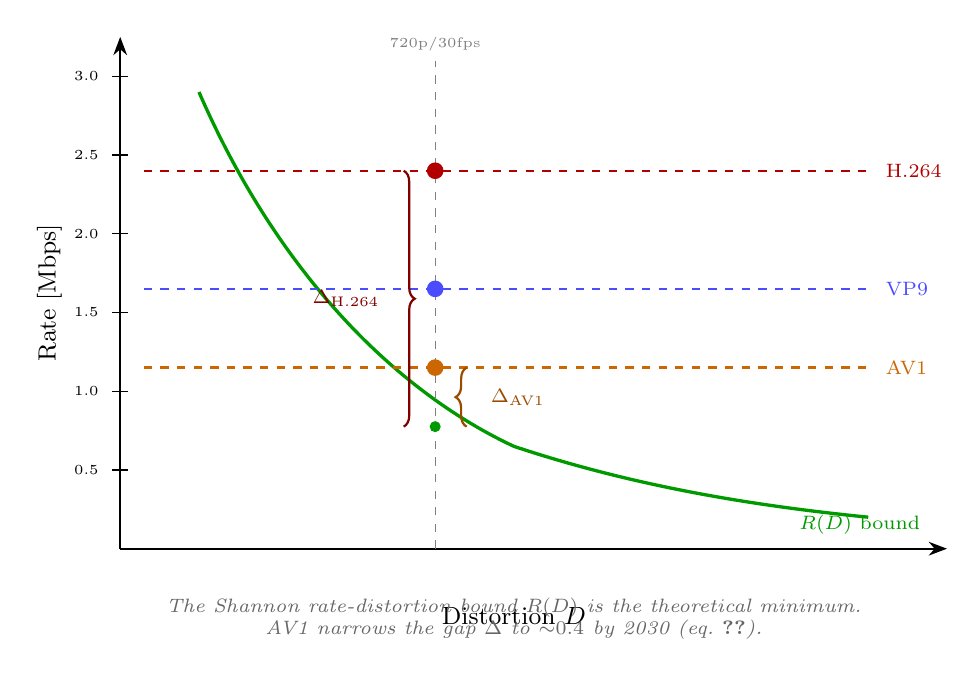
\begin{tikzpicture}[>=Stealth]

% --- Axes ---
\draw[->, thick] (0, 0) -- (10.5, 0);
\draw[->, thick] (0, 0) -- (0, 6.5);

% --- Axis titles ---
\node[font=\small] at (5, -0.85) {Distortion $D$};
\node[font=\small, rotate=90] at (-0.9, 3.25) {Rate [Mbps]};

% --- Y-axis rate labels ---
\foreach \y/\lab in {1.0/0.5, 2.0/1.0, 3.0/1.5, 4.0/2.0, 5.0/2.5, 6.0/3.0} {
  \draw (-0.1, \y) -- (0.1, \y);
  \node[font=\tiny, anchor=east] at (-0.15, \y) {\lab};
}

% --- R(D) Shannon bound curve ---
\draw[very thick, green!60!black]
  (1.0, 5.8) .. controls (2.0, 3.5) and (3.5, 2.0) ..
  (5.0, 1.3) .. controls (6.5, 0.8) and (8.0, 0.55) ..
  (9.5, 0.4);
\node[font=\scriptsize, green!60!black, anchor=north west] at (8.5, 0.55)
  {$R(D)$ bound};

% --- Reference distortion line (720p/30fps operating point) ---
\draw[thin, gray, dashed] (4.0, 0) -- (4.0, 6.2);
\node[font=\tiny, gray, anchor=south] at (4.0, 6.2) {720p/30fps};

% --- R(D) value at reference distortion ---
\fill[green!60!black] (4.0, 1.55) circle (2pt);

% --- Codec operating points at reference distortion ---
% H.264: ~2.5 Mbps
\draw[thick, dashed, red!70!black] (0.3, 4.8) -- (9.5, 4.8);
\fill[red!70!black] (4.0, 4.8) circle (3pt);
\node[font=\scriptsize, red!70!black, anchor=west] at (9.6, 4.8) {H.264};

% VP9: ~1.6 Mbps (0.65 * H.264)
\draw[thick, dashed, blue!70] (0.3, 3.3) -- (9.5, 3.3);
\fill[blue!70] (4.0, 3.3) circle (3pt);
\node[font=\scriptsize, blue!70, anchor=west] at (9.6, 3.3) {VP9};

% AV1: ~1.15 Mbps (0.46 * H.264)
\draw[thick, dashed, orange!80!black] (0.3, 2.3) -- (9.5, 2.3);
\fill[orange!80!black] (4.0, 2.3) circle (3pt);
\node[font=\scriptsize, orange!80!black, anchor=west] at (9.6, 2.3) {AV1};

% --- Gap annotations (braces) ---
% H.264 gap
\draw[decorate, decoration={brace, amplitude=4pt, mirror},
  thick, red!50!black]
  (3.6, 1.55) -- (3.6, 4.8)
  node[midway, anchor=east, font=\scriptsize, xshift=-5pt]
  {$\Delta_{\text{H.264}}$};

% AV1 gap
\draw[decorate, decoration={brace, amplitude=4pt},
  thick, orange!60!black]
  (4.4, 1.55) -- (4.4, 2.3)
  node[midway, anchor=west, font=\scriptsize, xshift=5pt]
  {$\Delta_{\text{AV1}}$};

% --- Annotation ---
\node[font=\scriptsize\itshape, text=black!60, align=center,
  anchor=north] at (5.0, -0.5)
  {The Shannon rate-distortion bound $R(D)$ is the theoretical minimum.\\
   AV1 narrows the gap $\Delta$ to ${\sim}0.4$ by 2030 (eq.~\ref{eq:coding-gap}).};

\end{tikzpicture}
\caption{Codec operating rates vs.\ the Shannon rate-distortion bound $R(D)$
  at 720p/30fps. Each codec operates above the theoretical minimum; the gap
  $\Delta$ (eq.~\ref{eq:coding-gap}) shrinks from H.264 through VP9 to AV1,
  approaching but never reaching the bound.}
\label{fig:rate-distortion}
\end{figure}

\subsubsection{Codec Entropy and WebCodecs}

The WebCodecs API (W3C Working Draft) exposes per-frame codec access,
allowing measurement and control of the instantaneous encoding rate.
For a video frame $f_t$ at time $t$, the encoder output has empirical
entropy:
\begin{equation}
  \hat{H}(f_t) = -\sum_{s \in \mathcal{S}}
    p(s \mid f_t) \log_2 p(s \mid f_t)
  \label{eq:frame-entropy}
\end{equation}
where $\mathcal{S}$ is the set of symbols emitted by the entropy coder
(CABAC for H.264/AV1, arithmetic coding for VP9). WebCodecs enables
applications to observe $|E(f_t)|$ (the encoded frame size in bits)
directly, which serves as a practical upper bound on
$\hat{H}(f_t)$:
\begin{equation}
  \hat{H}(f_t) \leq |E(f_t)| \leq R_{\text{codec}} / \text{fps}
  \label{eq:entropy-bound}
\end{equation}

\subsection{Effective Information Rate by Time Horizon}

We now combine transport and source coding measures to estimate the
effective information rate for a representative real-time video
session: a single 720p/30fps video call with one audio channel.

\excursus{Excursus: Why 720p?}{Throughout this appendix, 720p/30fps is used as
a fixed reference for cross-era comparison, not as a prediction that 720p
remains the dominant conferencing resolution. The bandwidth surplus quantified
below is precisely what enables migration to 1080p (feasible by ${\sim}$2028
with AV1 hardware encode at today's 720p bit rates) and 4K (feasible by
${\sim}$2030). The 720p baseline makes the efficiency gains legible: the same
task gets cheaper, freeing capacity for higher quality or more streams.}

Define the \emph{net information rate} as:
\begin{equation}
  I_{\text{net}} = R_{\text{codec}} \cdot \eta_{\text{transport}}
    \cdot (1 - \rho_{\text{overhead}})
    \cdot (1 - p_{\text{loss}})
  \label{eq:inet}
\end{equation}

\begin{table}[ht]
\centering
\small
\renewcommand{\arraystretch}{1.4}
\begin{tabularx}{\textwidth}{lXXX}
\toprule
\textbf{Parameter} & \textbf{March 2026} & \textbf{2027--2028} &
  \textbf{2029--2031} \\
\midrule
Median link capacity &
  120~Mbps &
  $\sim$150~Mbps &
  200--300~Mbps \\
Dominant codec (WebRTC) &
  VP9 / H.264 &
  VP9 / AV1 (HW) &
  AV1 (HW default) \\
Codec rate (720p/30fps) &
  1.5--2.5~Mbps &
  1.0--1.8~Mbps &
  0.7--1.2~Mbps \\
$\eta_{\text{transport}}$ &
  0.92 (QUIC) &
  0.93 &
  0.94 \\
$\rho_{\text{overhead}}$ (SRTP+QUIC) &
  0.06 &
  0.05 &
  0.04 \\
Typical loss $p$ &
  0.01--0.03 &
  0.01--0.02 &
  0.005--0.01 \\
$I_{\text{net}}$ (720p video) &
  1.3--2.2~Mbps &
  0.9--1.6~Mbps &
  0.6--1.1~Mbps \\
$I_{\text{net}}$ as \% of $C_{\text{link}}$ &
  1.1--1.8\% &
  0.6--1.1\% &
  0.2--0.6\% \\
\bottomrule
\end{tabularx}
\caption{Effective information rate for a 720p/30fps WebRTC video stream.
  The declining ratio $I_{\text{net}} / C_{\text{link}}$ reflects both
  improved codec efficiency and growing link capacity, freeing bandwidth
  for higher resolutions, additional streams, or concurrent data
  channels.}
\label{tab:inet}
\end{table}

The declining ratio $I_{\text{net}} / C_{\text{link}}$ in
Table~\ref{tab:inet} is the central quantitative observation: by 2030, a
720p video call consumes less than 0.5\% of available link capacity. The
surplus capacity enables qualitative changes --- 4K video conferencing,
multi-stream layouts, or concurrent data channels via WebTransport ---
that are quantitatively infeasible in 2026.

\begin{figure}[ht]
\centering
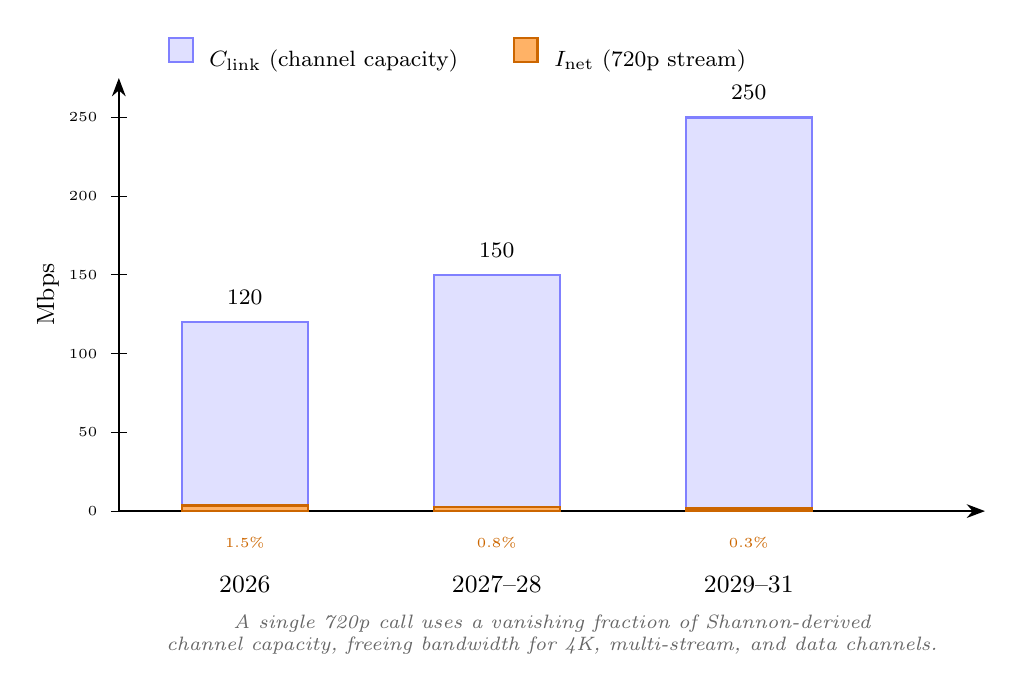
\begin{tikzpicture}[>=Stealth]

% --- Axes ---
\draw[->, thick] (0, 0) -- (11, 0);
\draw[->, thick] (0, 0) -- (0, 5.5);

% --- Axis title ---
\node[font=\small, rotate=90] at (-0.9, 2.75) {Mbps};

% --- Y-axis labels ---
\foreach \y/\lab in {0/0, 1/50, 2/100, 3/150, 4/200, 5/250} {
  \draw (-0.1, \y) -- (0.1, \y);
  \node[font=\tiny, anchor=east] at (-0.15, \y) {\lab};
}

% --- Group: March 2026 ---
% C_link = 120 Mbps -> y = 2.4
\fill[blue!12] (0.8, 0) rectangle (2.4, 2.4);
\draw[blue!50, thick] (0.8, 0) rectangle (2.4, 2.4);
% I_net = 1.75 Mbps (midpoint) -> y = 0.035
\fill[orange!60] (0.8, 0) rectangle (2.4, 0.07);
\draw[orange!80!black, thick] (0.8, 0) rectangle (2.4, 0.07);
\node[font=\footnotesize, anchor=south] at (1.6, 2.5) {120};
\node[font=\tiny, orange!80!black] at (1.6, -0.4) {1.5\%};
\node[font=\small, anchor=north] at (1.6, -0.7) {2026};

% --- Group: 2027--2028 ---
% C_link = 150 Mbps -> y = 3.0
\fill[blue!12] (4.0, 0) rectangle (5.6, 3.0);
\draw[blue!50, thick] (4.0, 0) rectangle (5.6, 3.0);
% I_net = 1.25 Mbps (midpoint) -> y = 0.025
\fill[orange!60] (4.0, 0) rectangle (5.6, 0.05);
\draw[orange!80!black, thick] (4.0, 0) rectangle (5.6, 0.05);
\node[font=\footnotesize, anchor=south] at (4.8, 3.1) {150};
\node[font=\tiny, orange!80!black] at (4.8, -0.4) {0.8\%};
\node[font=\small, anchor=north] at (4.8, -0.7) {2027--28};

% --- Group: 2029--2031 ---
% C_link = 250 Mbps -> y = 5.0
\fill[blue!12] (7.2, 0) rectangle (8.8, 5.0);
\draw[blue!50, thick] (7.2, 0) rectangle (8.8, 5.0);
% I_net = 0.85 Mbps (midpoint) -> y = 0.017
\fill[orange!60] (7.2, 0) rectangle (8.8, 0.034);
\draw[orange!80!black, thick] (7.2, 0) rectangle (8.8, 0.034);
\node[font=\footnotesize, anchor=south] at (8.0, 5.1) {250};
\node[font=\tiny, orange!80!black] at (8.0, -0.4) {0.3\%};
\node[font=\small, anchor=north] at (8.0, -0.7) {2029--31};

% --- Legend ---
\node[anchor=west, font=\footnotesize] at (0.5, 5.8) {%
  \tikz[baseline=-0.5ex]{\fill[blue!12] (0,0) rectangle (0.3,0.3);
    \draw[blue!50, thick] (0,0) rectangle (0.3,0.3);}
  ~$C_{\text{link}}$ (channel capacity) \qquad
  \tikz[baseline=-0.5ex]{\fill[orange!60] (0,0) rectangle (0.3,0.3);
    \draw[orange!80!black, thick] (0,0) rectangle (0.3,0.3);}
  ~$I_{\text{net}}$ (720p stream)};

% --- Annotation ---
\node[font=\scriptsize\itshape, text=black!60, align=center,
  anchor=north] at (5.5, -1.2)
  {A single 720p call uses a vanishing fraction of Shannon-derived\\
   channel capacity, freeing bandwidth for 4K, multi-stream, and data channels.};

\end{tikzpicture}
\caption{Channel capacity $C_{\text{link}}$ vs.\ effective information rate
  $I_{\text{net}}$ for a single 720p/30fps stream across time horizons. The
  orange bar (stream rate) is barely visible against the blue bar (capacity),
  illustrating the growing surplus as codecs improve and bandwidth increases.}
\label{fig:inet-capacity}
\end{figure}

\subsection{Security Entropy and Key Space}

The DTLS-SRTP security architecture (RFCs~8827, 3711) protects all
WebRTC media. Information-theoretic security requires that the key
entropy exceed the information content of the protected material.

For a DTLS~1.3 handshake with ECDHE on P-256, the key agreement
provides:
\begin{equation}
  H_{\text{key}} = 128 \text{~bits of security}
  \label{eq:key-entropy}
\end{equation}

The SRTP master key is 128 bits (AES-128-GCM), giving an exhaustive
search cost of $2^{128}$ operations. The total information content of a
one-hour 720p video call at 2~Mbps is:
\begin{equation}
  I_{\text{call}} = 2 \times 10^6 \times 3600
    = 7.2 \times 10^9 \text{~bits}
    \approx 2^{32.7} \text{~bits}
  \label{eq:call-content}
\end{equation}

The ratio of key entropy to protected content:
\begin{equation}
  \frac{H_{\text{key}}}{I_{\text{call}}}
    = \frac{128}{32.7} \approx 3.91
  \label{eq:security-margin}
\end{equation}

This ratio remains comfortably above~1 even for much longer sessions.
For a continuous 24-hour 4K AV1 stream at 15~Mbps:
\begin{equation}
  I_{\text{stream}} = 15 \times 10^6 \times 86400
    = 1.296 \times 10^{12} \text{~bits}
    \approx 2^{40.2} \text{~bits}
\end{equation}
yielding $H_{\text{key}} / I_{\text{stream}} \approx 3.18$, still
well above the threshold.

\subsubsection{End-to-End Encryption via Encoded Transforms}

The RTCRtpScriptTransform API (Encoded Transforms) enables
application-layer E2EE within the WebRTC pipeline. From an
information-theoretic perspective, this introduces a second encryption
layer with its own key, creating a \emph{nested channel}:
\begin{equation}
  X \xrightarrow{\;K_{\text{E2EE}}\;}
  E_1(X) \xrightarrow{\;K_{\text{SRTP}}\;}
  E_2(E_1(X))
  \label{eq:nested}
\end{equation}

The mutual information between the ciphertext and plaintext, given
neither key, satisfies:
\begin{equation}
  I\!\left(X;\, E_2(E_1(X))\right) \leq
    \min\!\big(H(K_{\text{E2EE}})^{-1},\;
    H(K_{\text{SRTP}})^{-1}\big)
    \cdot I_{\text{call}}
  \label{eq:mutual-e2ee}
\end{equation}

In practice, with $H(K_{\text{E2EE}}) = H(K_{\text{SRTP}}) = 128$
bits, this quantity is negligible ($\ll 1$ bit for any practical
session length), confirming that the nested encryption provides
information-theoretic confidentiality well beyond computational
security guarantees.

Today (March~2026), Encoded Transforms remain Chrome-only. By
2027--2028 (Section~8.3), cross-browser standardization will make
this nested channel universally available. By 2029--2031, SFrame
for group calls will extend this to $n$-party sessions, where the
mutual information between any non-member and the group plaintext
remains negligible:
\begin{equation}
  I\!\left(X;\, E(X) \;\middle|\; K_i \notin
    \{K_1, \ldots, K_n\}\right) \approx 0
  \label{eq:sframe}
\end{equation}

\subsection{WebTransport: Unreliable Datagrams and Channel Capacity}

WebTransport (RFC~9297) introduces unreliable datagrams to browser-server
communication. For latency-sensitive applications (game state, sensor
telemetry), the relevant measure is not throughput but
\emph{freshness-weighted information rate}. Define the value of a
datagram as exponentially decaying with delivery latency $\delta$:
\begin{equation}
  V(\delta) = e^{-\lambda \delta}
  \label{eq:freshness}
\end{equation}
where $\lambda > 0$ is an application-specific decay rate. The
effective information rate under unreliable delivery is:
\begin{equation}
  I_{\text{WT}} = R_{\text{send}} \cdot (1 - p_{\text{loss}})
    \cdot \mathbb{E}\!\left[e^{-\lambda \delta}\right]
  \label{eq:iwt}
\end{equation}

Under reliable delivery (TCP/WebSocket), a retransmission delays
subsequent data, so:
\begin{equation}
  I_{\text{WS}} = R_{\text{send}}
    \cdot \mathbb{E}\!\left[e^{-\lambda(\delta + p \cdot 2\tau)}\right]
  \label{eq:iws}
\end{equation}

The ratio $I_{\text{WT}} / I_{\text{WS}}$ exceeds 1 when:
\begin{equation}
  (1 - p) \cdot e^{\lambda \cdot p \cdot 2\tau} > 1
  \quad \Longleftrightarrow \quad
  \lambda > \frac{-\ln(1 - p)}{2 p \tau}
  \label{eq:wt-advantage}
\end{equation}

For $p = 0.02$ and $\tau = 25$~ms, this gives $\lambda > 20.2$~s$^{-1}$
(half-life $< 34$~ms).

\excursus{Excursus: Why $p = 0.02$ and $\tau = 25$\,ms?}{These values represent
median fixed-broadband conditions in 2026 (Table~\ref{tab:inet}). On mobile or
congested links ($p \approx 0.05$, $\tau \approx 50$\,ms), the threshold
$\lambda^*$ drops to ${\sim}10$\,s$^{-1}$, broadening WebTransport's advantage
to applications with data half-lives up to ${\sim}70$\,ms. The fixed-broadband
reference is thus conservative: mobile scenarios favor unreliable delivery even
more strongly.}

Any application where data older than
$\sim$30~ms is useless benefits from WebTransport's unreliable
mode over WebSocket --- precisely the regime of interactive gaming, live
cursor tracking, and real-time sensor feeds.

As of March~2026, Safari does not support WebTransport
(Section~5), limiting coverage to $\sim$82\%. By 2027--2028
(Section~8.2), universal support will allow applications to rely on
(\ref{eq:iwt}) without fallback paths.

\begin{figure}[ht]
\centering
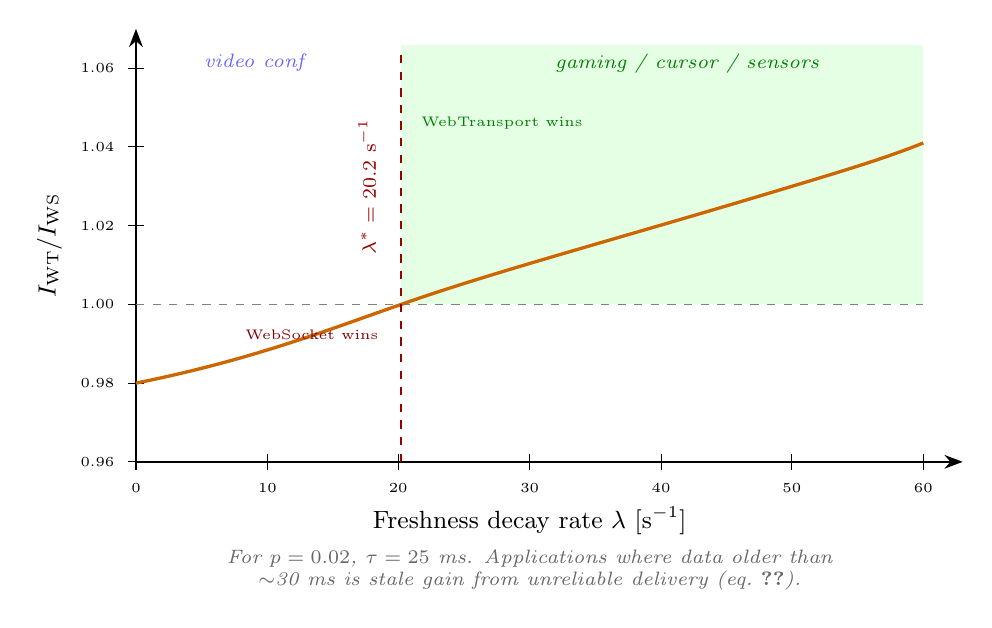
\begin{tikzpicture}[>=Stealth]

% --- Axes ---
\draw[->, thick] (0, 0) -- (10.5, 0);
\draw[->, thick] (0, 0) -- (0, 5.5);

% --- Axis titles (positioned to clear tick labels) ---
\node[font=\small] at (5, -0.75)
  {Freshness decay rate $\lambda$ [s$^{-1}$]};
\node[font=\small, rotate=90] at (-1.1, 2.75)
  {$I_{\text{WT}} / I_{\text{WS}}$};

% --- X-axis labels ---
\foreach \x/\lab in {0/0, 1.67/10, 3.33/20, 5.0/30, 6.67/40, 8.33/50, 10/60} {
  \draw (\x, -0.1) -- (\x, 0.1);
  \node[font=\tiny, anchor=north] at (\x, -0.15) {\lab};
}

% --- Y-axis labels (0.96 to 1.06, each 0.02 = 1 unit) ---
\foreach \y/\lab in {0/0.96, 1/0.98, 2/1.00, 3/1.02, 4/1.04, 5/1.06} {
  \draw (-0.1, \y) -- (0.1, \y);
  \node[font=\tiny, anchor=east] at (-0.15, \y) {\lab};
}

% --- Ratio = 1.0 line (y=2 maps to ratio 1.0) ---
\draw[thin, gray, dashed] (0, 2) -- (10, 2);

% --- Shade WebTransport advantage region ---
% lambda* = 20.2 -> x = 3.37
\fill[green!10] (3.37, 2) rectangle (10, 5.3);

% --- I_WT/I_WS curve: 0.98*exp(lambda*0.001) ---
% Y range: 0.96-1.06 (each 0.02 = 1 unit). lambda=0: y=1, lambda*=20.2: y=2, lambda=60: y=4.05
\draw[very thick, orange!80!black]
  (0, 1.0) .. controls (1.5, 1.3) and (2.5, 1.7) ..
  (3.37, 2.0) .. controls (4.5, 2.4) and (6, 2.8) ..
  (8, 3.4) .. controls (9, 3.7) and (9.5, 3.85) ..
  (10, 4.05);

% --- Threshold line ---
\draw[thick, dashed, red!60!black] (3.37, 0) -- (3.37, 5.2);
\node[font=\scriptsize, red!60!black, anchor=south, rotate=90] at (3.17, 3.5)
  {$\lambda^* = 20.2$ s$^{-1}$};

% --- Application regime labels ---
\node[font=\scriptsize\itshape, text=blue!60, anchor=north] at (1.5, 5.3)
  {video conf};
\node[font=\scriptsize\itshape, text=green!50!black, anchor=north] at (7.0, 5.3)
  {gaming / cursor / sensors};

% --- Mark advantage/disadvantage ---
\node[font=\tiny, text=red!50!black, anchor=north east] at (3.2, 1.8)
  {WebSocket wins};
\node[font=\tiny, text=green!50!black, anchor=north west] at (3.5, 4.5)
  {WebTransport wins};

% --- Annotation ---
\node[font=\scriptsize\itshape, text=black!60, align=center,
  anchor=north] at (5.0, -1.0)
  {For $p = 0.02$, $\tau = 25$~ms. Applications where data older than\\
   ${\sim}$30~ms is stale gain from unreliable delivery (eq.~\ref{eq:wt-advantage}).};

\end{tikzpicture}
\caption{Freshness-weighted information rate ratio $I_{\text{WT}} / I_{\text{WS}}$
  as a function of decay rate $\lambda$. Above the threshold $\lambda^*$,
  WebTransport's unreliable datagrams deliver more useful information per
  unit time than WebSocket's reliable delivery, because retransmission
  wastes capacity on stale data.}
\label{fig:freshness}
\end{figure}

\subsection{Projections Summary and Practical Implications}

\begin{table}[ht]
\centering
\small
\renewcommand{\arraystretch}{1.4}
\begin{tabularx}{\textwidth}{lXXX}
\toprule
\textbf{Measure} & \textbf{March 2026} & \textbf{2027--2028} &
  \textbf{2029--2031} \\
\midrule
Channel capacity $C_{\text{link}}$ &
  120~Mbps &
  150~Mbps &
  250~Mbps \\
HOL blocking factor $(1\!-\!p)^{n-2}$ at $n\!=\!8$ &
  0.94 ($p\!=\!0.01$) &
  0.94 &
  0.97 ($p\!=\!0.005$) \\
Source coding gap $\Delta$ &
  VP9: $\sim$0.8 &
  AV1 HW: $\sim$0.5 &
  AV1 opt: $\sim$0.4 \\
$I_{\text{net}}$ per 720p stream &
  1.3--2.2~Mbps &
  0.9--1.6~Mbps &
  0.6--1.1~Mbps \\
Max 720p streams in $C_{\text{link}}$ &
  $\sim$55--90 &
  $\sim$95--165 &
  $\sim$230--415 \\
E2EE availability &
  Chrome only &
  Cross-browser &
  SFrame $n$-party \\
WebTransport coverage &
  82\% &
  $\sim$100\% &
  100\% \\
Freshness threshold $\lambda^*$ &
  20.2~s$^{-1}$ &
  $\sim$18~s$^{-1}$ &
  $\sim$15~s$^{-1}$ \\
\bottomrule
\end{tabularx}
\caption{Information-theoretic measures across time horizons. $\Delta$
  is the coding efficiency gap (\ref{eq:coding-gap}), $I_{\text{net}}$
  is the net information rate (\ref{eq:inet}), and $\lambda^*$ is the
  freshness decay threshold above which WebTransport dominates WebSocket
  (\ref{eq:wt-advantage}).}
\label{tab:projections}
\end{table}

The trajectory is clear: the combination of improving source coding
(AV1 hardware), expanding channel capacity (broadband growth), and
maturing transport protocols (QUIC universal, WebTransport universal)
drives the \emph{information cost per unit of communicated experience}
steadily downward. The remaining question is not whether the
Shannon capacity suffices --- it already does, by orders of magnitude
--- but how efficiently the protocol stack converts that capacity into
delivered, fresh, secure information at the application layer. By
2030, the gap between theoretical capacity and realized throughput will
be the narrowest it has ever been for browser-based real-time
communication.

\subsubsection{What the Theory Means for Applications}

The equations and figures in this appendix are not purely academic. Each
theoretical result maps to a concrete design decision that application
developers face today and over the next five years.

\textbf{Codec selection determines bandwidth cost, not quality.}
The rate-distortion analysis (Section~A.2, Figure~\ref{fig:rate-distortion})
shows that AV1 operates at roughly 46\% of H.264's bit rate for equivalent
perceptual quality at 720p. In practice, this means a WebRTC application
switching from H.264 to AV1 can either halve its bandwidth consumption at
the same quality or substantially increase resolution (e.g., 720p to 1080p)
within the same bandwidth envelope. By 2030, with AV1 hardware encoding
ubiquitous and the coding gap $\Delta$ approaching 0.4, further codec
improvements yield diminishing returns --- the stack will be operating close
enough to the Shannon rate-distortion bound that the next generation of
efficiency gains will come from transport and architecture, not codecs alone.

\textbf{QUIC's advantage is situational but decisive on bad networks.}
The head-of-line blocking analysis (Section~A.1.1,
Figure~\ref{fig:hol-blocking}) shows that QUIC's per-stream throughput
advantage over TCP is modest on good networks (6\% at 1\% loss) but
substantial on degraded ones (34\% at 5\% loss). The practical implication
is that applications targeting mobile users, emerging markets, or congested
enterprise networks --- precisely the environments where real-time
communication is hardest --- benefit disproportionately from QUIC-based
transports. For a video conference with 8 participants on a cellular
connection experiencing 3--5\% packet loss, the difference between QUIC and
TCP is the difference between usable and degraded video.

\textbf{Connection latency is a solved problem for returning users.}
The handshake analysis (Section~A.1.2) shows that QUIC 0-RTT eliminates
connection establishment overhead entirely for resumed connections. For a
WebTransport application that a user opens daily --- a collaboration tool,
a live dashboard, a recurring meeting client --- the time to first useful
byte drops to zero. The 1.125~MB of wasted capacity during a TCP+TLS
handshake on a 120~Mbps link may seem small, but for latency-sensitive
applications where the first 100~ms of perceived responsiveness determines
user experience, the difference is measurable.

\textbf{Bandwidth surplus enables architectural ambition.}
The effective information rate analysis (Section~A.3,
Figure~\ref{fig:inet-capacity}) reveals the most consequential practical
finding: a single 720p video stream consumes a vanishing fraction of
available link capacity (under 0.5\% by 2030). This surplus is not merely
``headroom'' --- it is the resource that makes new application architectures
feasible. A 250~Mbps link can theoretically carry 230--415 simultaneous 720p
streams. In practice, this means applications can afford to run multiple
concurrent media flows (video, screen share, spatial audio), data channels
(collaborative editing, file transfer), and telemetry streams without
contending for bandwidth. The constraint shifts from ``can the network carry
this?''\ to ``can the application manage this complexity?''

\textbf{End-to-end encryption adds negligible overhead.}
The security analysis (Section~A.4) confirms that the nested DTLS-SRTP plus
E2EE architecture imposes no meaningful information-theoretic cost. The key
entropy ($2^{128}$) exceeds the information content of any practical session
by a factor of at least 3. For application developers, this means E2EE can
be treated as a default rather than a premium feature --- there is no
bandwidth, latency, or capacity penalty for encrypting at the application
layer on top of the transport-layer encryption that WebRTC already mandates.
The only constraint is API availability, which moves from Chrome-only (2026)
to universal (2028).

\textbf{WebTransport unlocks real-time data that WebSocket cannot serve.}
The freshness analysis (Section~A.5, Figure~\ref{fig:freshness}) quantifies
when unreliable delivery outperforms reliable delivery: any data with a
useful half-life below approximately 34~ms benefits from WebTransport's
unreliable datagrams. This covers a wide class of interactive applications
--- game state synchronization, live cursor and pointer sharing, real-time
sensor feeds, collaborative whiteboard strokes --- where retransmitting a
stale update is worse than dropping it. Before WebTransport, these
applications had to choose between WebSocket (reliable but stale under loss)
and WebRTC DataChannel (unreliable mode available but requiring the full
peer-to-peer ICE/DTLS machinery). WebTransport provides the unreliable
mode with a simple client-server model over HTTP/3, removing the
architectural overhead.

\textbf{The overall picture: the stack converges on efficiency.}
Taken together, the information-theoretic measures trace a consistent
trajectory. The protocol stack is converging toward the theoretical limits
established by Shannon: codecs approach the rate-distortion bound, transports
eliminate unnecessary blocking and handshake overhead, and encryption adds
negligible cost. By 2030, the practical distance between what the standards
deliver and what information theory permits will be the smallest it has ever
been for browser-based real-time communication. The consequence for
application developers is that the infrastructure --- standards, hardware,
and networks --- will no longer be the binding constraint. The remaining
challenge is purely architectural: how to compose these efficient, universal
primitives into applications that fully exploit the capacity and low latency
they provide.

%
% Requires in the preamble: amsmath, amssymb, tabularx, booktabs

\section{Information-Theoretic View}
\label{app:info-theory}

This appendix applies information-theoretic measures to the real-time
web communication stack described in this document. We quantify channel
capacity, source coding efficiency, and effective information rates
across three time horizons: today (March~2026), the near term
(2027--2028), and the medium term (2029--2031). The analysis draws on
the standards, codec parameters, and infrastructure projections
developed in the main text.

\subsection{Channel Capacity of the Transport Layer}

The Shannon-Hartley theorem gives the theoretical maximum information
rate for a channel with additive white Gaussian noise:
\begin{equation}
  C = B \log_2\!\left(1 + \frac{S}{N}\right) \quad \text{[bits/s]}
  \label{eq:shannon}
\end{equation}
where $B$ is the channel bandwidth in Hz and $S/N$ is the
signal-to-noise ratio.

While the physical-layer capacity of a broadband link is governed by
(\ref{eq:shannon}), the \emph{effective} capacity available to the
application is reduced by protocol overhead, congestion control, and
transport inefficiencies. We define the effective application-layer
throughput as:
\begin{equation}
  R_{\text{eff}} = C_{\text{link}} \cdot \eta_{\text{transport}}
    \cdot (1 - \rho_{\text{overhead}})
  \label{eq:reff}
\end{equation}
where $C_{\text{link}}$ is the link-layer capacity,
$\eta_{\text{transport}} \in (0,1]$ is the transport efficiency factor
(capturing congestion control, retransmission, and multiplexing
behavior), and $\rho_{\text{overhead}} \in [0,1)$ is the fractional
protocol overhead (headers, encryption, framing).

\subsubsection{Head-of-Line Blocking and Multiplexed Capacity}

Consider $n$ independent streams multiplexed over a single connection.
Under TCP (HTTP/2), a single lost packet blocks all $n$ streams. The
expected throughput per stream under loss rate $p$ is bounded by:
\begin{equation}
  R_{\text{TCP}}^{(i)} \leq \frac{R_{\text{eff}}}{n}
    \cdot (1 - p)^{n-1}
  \label{eq:hol-tcp}
\end{equation}
because a loss in \emph{any} of the $n$ streams stalls all others. Under
QUIC (RFC~9000), streams are independent at the transport layer, so:
\begin{equation}
  R_{\text{QUIC}}^{(i)} \leq \frac{R_{\text{eff}}}{n}
    \cdot (1 - p)
  \label{eq:hol-quic}
\end{equation}
The ratio of effective per-stream throughput is:
\begin{equation}
  \frac{R_{\text{QUIC}}^{(i)}}{R_{\text{TCP}}^{(i)}}
    = \frac{1}{(1-p)^{n-2}}
  \label{eq:hol-ratio}
\end{equation}
\excursus{Excursus: Why $n = 8$?}{In a typical multi-participant video
conference, each peer contributes multiple concurrent streams: a camera video
track, an audio track, and often a screen-share or data channel. A four-person
call with two media tracks each produces $n = 8$ multiplexed streams over a
single connection --- the reference value used throughout this section. Larger
meetings (e.g.\ 10 participants with simulcast layers) push $n$ higher,
amplifying the HOL blocking effect further.}

For $n = 8$ streams (a typical multi-track video conference) at
$p = 0.01$ (1\% loss), this gives a QUIC advantage factor of
$1/(0.99)^6 \approx 1.062$, a modest 6.2\% improvement. At $p = 0.05$
(5\% loss, common on mobile or congested links), the factor is
$1/(0.95)^6 \approx 1.34$, a 34\% throughput advantage per stream.

\begin{figure}[ht]
\centering
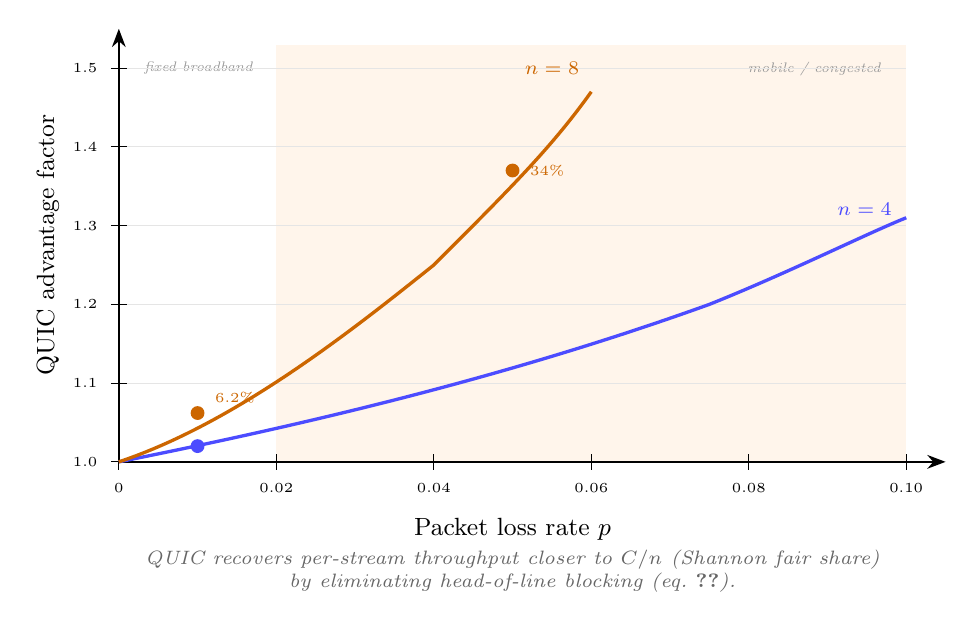
\begin{tikzpicture}[>=Stealth]

% --- Shaded region (drawn FIRST so curves appear on top) ---
\fill[orange!8] (2, 0) rectangle (10, 5.3);
\node[font=\tiny\itshape, text=black!40, anchor=north east] at (9.8, 5.2)
  {mobile / congested};
\node[font=\tiny\itshape, text=black!40, anchor=north west] at (0.2, 5.2)
  {fixed broadband};

% --- Grid lines ---
\foreach \y in {1, 2, 3, 4, 5} {
  \draw[gray!20] (0, \y) -- (10, \y);
}

% --- Axes ---
\draw[->, thick] (0, 0) -- (10.5, 0);
\draw[->, thick] (0, 0) -- (0, 5.5);

% --- Axis titles (positioned to clear tick labels) ---
\node[font=\small] at (5, -0.85) {Packet loss rate $p$};
\node[font=\small, rotate=90] at (-0.9, 2.75) {QUIC advantage factor};

% --- X-axis labels ---
\foreach \x/\lab in {0/0, 2/0.02, 4/0.04, 6/0.06, 8/0.08, 10/0.10} {
  \draw (\x, -0.1) -- (\x, 0.1);
  \node[font=\tiny, anchor=north] at (\x, -0.15) {\lab};
}

% --- Y-axis labels ---
\foreach \y/\lab in {0/1.0, 1/1.1, 2/1.2, 3/1.3, 4/1.4, 5/1.5} {
  \draw (-0.1, \y) -- (0.1, \y);
  \node[font=\tiny, anchor=east] at (-0.15, \y) {\lab};
}

% --- n=4 curve: 1/(1-p)^2 ---
\draw[very thick, blue!70]
  (0, 0) .. controls (2.5, 0.5) and (5, 1.1) ..
  (7.5, 2.0) .. controls (8.5, 2.4) and (9.5, 2.9) ..
  (10, 3.1);
\node[font=\scriptsize, blue!70, anchor=south west] at (9.0, 3.0)
  {$n = 4$};

% --- n=8 curve: 1/(1-p)^6 ---
\draw[very thick, orange!80!black]
  (0, 0) .. controls (1.5, 0.5) and (3, 1.7) ..
  (4, 2.5) .. controls (5, 3.5) and (5.5, 4.0) ..
  (6, 4.7);
\node[font=\scriptsize, orange!80!black, anchor=south] at (5.5, 4.8)
  {$n = 8$};

% --- Reference points ---
\fill[orange!80!black] (1.0, 0.62) circle (2.5pt);
\node[font=\tiny, orange!80!black, anchor=south west] at (1.1, 0.62)
  {6.2\%};

\fill[orange!80!black] (5.0, 3.7) circle (2.5pt);
\node[font=\tiny, orange!80!black, anchor=west] at (5.1, 3.7)
  {34\%};

\fill[blue!70] (1.0, 0.20) circle (2.5pt);

% --- Annotation ---
\node[font=\scriptsize\itshape, text=black!60, align=center,
  anchor=north] at (5.0, -1.0)
  {QUIC recovers per-stream throughput closer to $C/n$ (Shannon fair share)\\
   by eliminating head-of-line blocking (eq.~\ref{eq:hol-ratio}).};

\end{tikzpicture}
\caption{QUIC advantage factor $1/(1-p)^{n-2}$ over TCP for multiplexed
  streams. At 5\% loss with $n=8$ streams, QUIC delivers 34\% more
  per-stream throughput by maintaining independence at the transport layer.}
\label{fig:hol-blocking}
\end{figure}

\subsubsection{Connection Establishment Latency}

Let $\tau$ denote the one-way latency (half the round-trip time). The
information-carrying capacity during connection establishment is zero;
the handshake represents pure overhead. The time to first useful byte
is:
\begin{align}
  T_{\text{TCP+TLS\,1.3}} &= 2\tau_{\text{TCP}} + \tau_{\text{TLS}}
    = 3\tau \quad \text{(1-RTT TLS~1.3)} \label{eq:tcp-setup} \\
  T_{\text{QUIC}} &= \tau \quad \text{(1-RTT)}
    \label{eq:quic-setup} \\
  T_{\text{QUIC,\,0-RTT}} &= 0 \quad \text{(resumption)}
    \label{eq:quic-0rtt}
\end{align}
The QUIC 0-RTT case (\ref{eq:quic-0rtt}) eliminates the handshake
entirely for resumed connections. The information lost during
handshake dead time, relative to steady-state capacity, is:
\begin{equation}
  I_{\text{lost}} = C_{\text{link}} \cdot T_{\text{setup}}
  \label{eq:ilost}
\end{equation}
For a 120~Mbps link with $\tau = 25$~ms (typical fixed broadband in
2026), the TCP+TLS~1.3 handshake wastes $120 \times 10^6 \times 0.075
= 9 \times 10^6$ bits (1.125~MB), while QUIC~1-RTT wastes only
$3 \times 10^6$ bits (375~KB).

\subsection{Source Coding Efficiency}

The rate-distortion function $R(D)$ defines the minimum bit rate
required to represent a source at distortion level $D$. For a
Gaussian source with variance $\sigma^2$ under mean squared error
distortion:
\begin{equation}
  R(D) = \frac{1}{2} \log_2 \frac{\sigma^2}{D}
    \quad \text{[bits/sample]}
  \label{eq:rate-distortion}
\end{equation}

\excursus{Excursus: Why Gaussian source?}{The Gaussian memoryless model is used
because it yields the highest (worst-case) $R(D)$ among all sources of equal
variance. Any codec that approaches the Gaussian bound on real video is
therefore doing at least as well as the bound predicts --- the true $R(D)$ for
spatially and temporally correlated video lies below the Gaussian curve, making
it a conservative benchmark.}

No practical codec achieves $R(D)$;\footnote{The $R(D)$ curve in
Figure~\ref{fig:rate-distortion} is the Gaussian memoryless source bound
(equation~\ref{eq:rate-distortion}), which is an upper bound on the true
$R(D)$ for non-Gaussian sources such as video.  Additionally, $R(D)$ assumes
zero excess-distortion probability, whereas practical codecs permit a
frame-level excess-distortion probability on the order of $10^{-6}$ to
$10^{-8}$.  Both factors allow codec operating points measured on real content
to approach or marginally cross the Gaussian bound.} real codecs operate at
some rate $R_{\text{codec}} > R(D)$. We define the coding efficiency gap as:
\begin{equation}
  \Delta = \frac{R_{\text{codec}} - R(D)}{R(D)}
  \label{eq:coding-gap}
\end{equation}

The codecs in the WebRTC stack can be ordered by their empirical
proximity to $R(D)$ for typical video content at conversational
resolutions (720p, 30~fps). Using published Bj\o ntegaard Delta (BD)
rate measurements:
\begin{equation}
  R_{\text{H.264}} > R_{\text{VP9}} > R_{\text{AV1}}
    > R(D)
  \label{eq:codec-ordering}
\end{equation}

Specifically, the empirical rate savings at equivalent PSNR are
approximately:
\begin{align}
  R_{\text{VP9}}  &\approx 0.65 \cdot R_{\text{H.264}}
    \quad (\sim\!35\% \text{ savings}) \label{eq:vp9-savings} \\
  R_{\text{AV1}}  &\approx 0.70 \cdot R_{\text{VP9}}
    \approx 0.46 \cdot R_{\text{H.264}}
    \quad (\sim\!30\% \text{ over VP9})
  \label{eq:av1-savings}
\end{align}

\begin{figure}[ht]
\centering
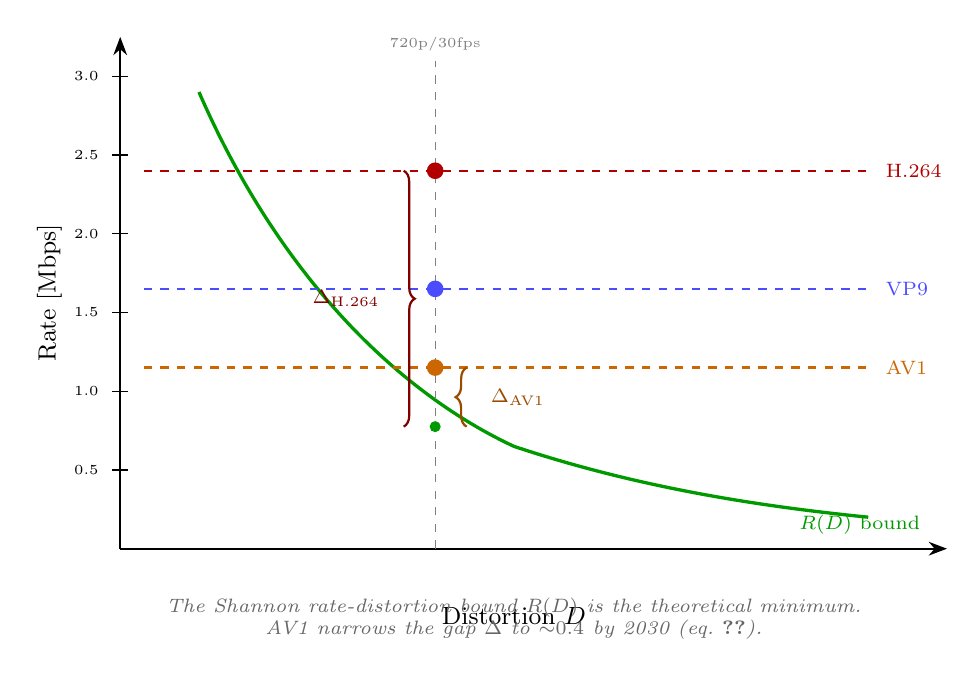
\begin{tikzpicture}[>=Stealth]

% --- Axes ---
\draw[->, thick] (0, 0) -- (10.5, 0);
\draw[->, thick] (0, 0) -- (0, 6.5);

% --- Axis titles ---
\node[font=\small] at (5, -0.85) {Distortion $D$};
\node[font=\small, rotate=90] at (-0.9, 3.25) {Rate [Mbps]};

% --- Y-axis rate labels ---
\foreach \y/\lab in {1.0/0.5, 2.0/1.0, 3.0/1.5, 4.0/2.0, 5.0/2.5, 6.0/3.0} {
  \draw (-0.1, \y) -- (0.1, \y);
  \node[font=\tiny, anchor=east] at (-0.15, \y) {\lab};
}

% --- R(D) Shannon bound curve ---
\draw[very thick, green!60!black]
  (1.0, 5.8) .. controls (2.0, 3.5) and (3.5, 2.0) ..
  (5.0, 1.3) .. controls (6.5, 0.8) and (8.0, 0.55) ..
  (9.5, 0.4);
\node[font=\scriptsize, green!60!black, anchor=north west] at (8.5, 0.55)
  {$R(D)$ bound};

% --- Reference distortion line (720p/30fps operating point) ---
\draw[thin, gray, dashed] (4.0, 0) -- (4.0, 6.2);
\node[font=\tiny, gray, anchor=south] at (4.0, 6.2) {720p/30fps};

% --- R(D) value at reference distortion ---
\fill[green!60!black] (4.0, 1.55) circle (2pt);

% --- Codec operating points at reference distortion ---
% H.264: ~2.5 Mbps
\draw[thick, dashed, red!70!black] (0.3, 4.8) -- (9.5, 4.8);
\fill[red!70!black] (4.0, 4.8) circle (3pt);
\node[font=\scriptsize, red!70!black, anchor=west] at (9.6, 4.8) {H.264};

% VP9: ~1.6 Mbps (0.65 * H.264)
\draw[thick, dashed, blue!70] (0.3, 3.3) -- (9.5, 3.3);
\fill[blue!70] (4.0, 3.3) circle (3pt);
\node[font=\scriptsize, blue!70, anchor=west] at (9.6, 3.3) {VP9};

% AV1: ~1.15 Mbps (0.46 * H.264)
\draw[thick, dashed, orange!80!black] (0.3, 2.3) -- (9.5, 2.3);
\fill[orange!80!black] (4.0, 2.3) circle (3pt);
\node[font=\scriptsize, orange!80!black, anchor=west] at (9.6, 2.3) {AV1};

% --- Gap annotations (braces) ---
% H.264 gap
\draw[decorate, decoration={brace, amplitude=4pt, mirror},
  thick, red!50!black]
  (3.6, 1.55) -- (3.6, 4.8)
  node[midway, anchor=east, font=\scriptsize, xshift=-5pt]
  {$\Delta_{\text{H.264}}$};

% AV1 gap
\draw[decorate, decoration={brace, amplitude=4pt},
  thick, orange!60!black]
  (4.4, 1.55) -- (4.4, 2.3)
  node[midway, anchor=west, font=\scriptsize, xshift=5pt]
  {$\Delta_{\text{AV1}}$};

% --- Annotation ---
\node[font=\scriptsize\itshape, text=black!60, align=center,
  anchor=north] at (5.0, -0.5)
  {The Shannon rate-distortion bound $R(D)$ is the theoretical minimum.\\
   AV1 narrows the gap $\Delta$ to ${\sim}0.4$ by 2030 (eq.~\ref{eq:coding-gap}).};

\end{tikzpicture}
\caption{Codec operating rates vs.\ the Shannon rate-distortion bound $R(D)$
  at 720p/30fps. Each codec operates above the theoretical minimum; the gap
  $\Delta$ (eq.~\ref{eq:coding-gap}) shrinks from H.264 through VP9 to AV1,
  approaching but never reaching the bound.}
\label{fig:rate-distortion}
\end{figure}

\subsubsection{Codec Entropy and WebCodecs}

The WebCodecs API (W3C Working Draft) exposes per-frame codec access,
allowing measurement and control of the instantaneous encoding rate.
For a video frame $f_t$ at time $t$, the encoder output has empirical
entropy:
\begin{equation}
  \hat{H}(f_t) = -\sum_{s \in \mathcal{S}}
    p(s \mid f_t) \log_2 p(s \mid f_t)
  \label{eq:frame-entropy}
\end{equation}
where $\mathcal{S}$ is the set of symbols emitted by the entropy coder
(CABAC for H.264/AV1, arithmetic coding for VP9). WebCodecs enables
applications to observe $|E(f_t)|$ (the encoded frame size in bits)
directly, which serves as a practical upper bound on
$\hat{H}(f_t)$:
\begin{equation}
  \hat{H}(f_t) \leq |E(f_t)| \leq R_{\text{codec}} / \text{fps}
  \label{eq:entropy-bound}
\end{equation}

\subsection{Effective Information Rate by Time Horizon}

We now combine transport and source coding measures to estimate the
effective information rate for a representative real-time video
session: a single 720p/30fps video call with one audio channel.

\excursus{Excursus: Why 720p?}{Throughout this appendix, 720p/30fps is used as
a fixed reference for cross-era comparison, not as a prediction that 720p
remains the dominant conferencing resolution. The bandwidth surplus quantified
below is precisely what enables migration to 1080p (feasible by ${\sim}$2028
with AV1 hardware encode at today's 720p bit rates) and 4K (feasible by
${\sim}$2030). The 720p baseline makes the efficiency gains legible: the same
task gets cheaper, freeing capacity for higher quality or more streams.}

Define the \emph{net information rate} as:
\begin{equation}
  I_{\text{net}} = R_{\text{codec}} \cdot \eta_{\text{transport}}
    \cdot (1 - \rho_{\text{overhead}})
    \cdot (1 - p_{\text{loss}})
  \label{eq:inet}
\end{equation}

\begin{table}[ht]
\centering
\small
\renewcommand{\arraystretch}{1.4}
\begin{tabularx}{\textwidth}{lXXX}
\toprule
\textbf{Parameter} & \textbf{March 2026} & \textbf{2027--2028} &
  \textbf{2029--2031} \\
\midrule
Median link capacity &
  120~Mbps &
  $\sim$150~Mbps &
  200--300~Mbps \\
Dominant codec (WebRTC) &
  VP9 / H.264 &
  VP9 / AV1 (HW) &
  AV1 (HW default) \\
Codec rate (720p/30fps) &
  1.5--2.5~Mbps &
  1.0--1.8~Mbps &
  0.7--1.2~Mbps \\
$\eta_{\text{transport}}$ &
  0.92 (QUIC) &
  0.93 &
  0.94 \\
$\rho_{\text{overhead}}$ (SRTP+QUIC) &
  0.06 &
  0.05 &
  0.04 \\
Typical loss $p$ &
  0.01--0.03 &
  0.01--0.02 &
  0.005--0.01 \\
$I_{\text{net}}$ (720p video) &
  1.3--2.2~Mbps &
  0.9--1.6~Mbps &
  0.6--1.1~Mbps \\
$I_{\text{net}}$ as \% of $C_{\text{link}}$ &
  1.1--1.8\% &
  0.6--1.1\% &
  0.2--0.6\% \\
\bottomrule
\end{tabularx}
\caption{Effective information rate for a 720p/30fps WebRTC video stream.
  The declining ratio $I_{\text{net}} / C_{\text{link}}$ reflects both
  improved codec efficiency and growing link capacity, freeing bandwidth
  for higher resolutions, additional streams, or concurrent data
  channels.}
\label{tab:inet}
\end{table}

The declining ratio $I_{\text{net}} / C_{\text{link}}$ in
Table~\ref{tab:inet} is the central quantitative observation: by 2030, a
720p video call consumes less than 0.5\% of available link capacity. The
surplus capacity enables qualitative changes --- 4K video conferencing,
multi-stream layouts, or concurrent data channels via WebTransport ---
that are quantitatively infeasible in 2026.

\begin{figure}[ht]
\centering
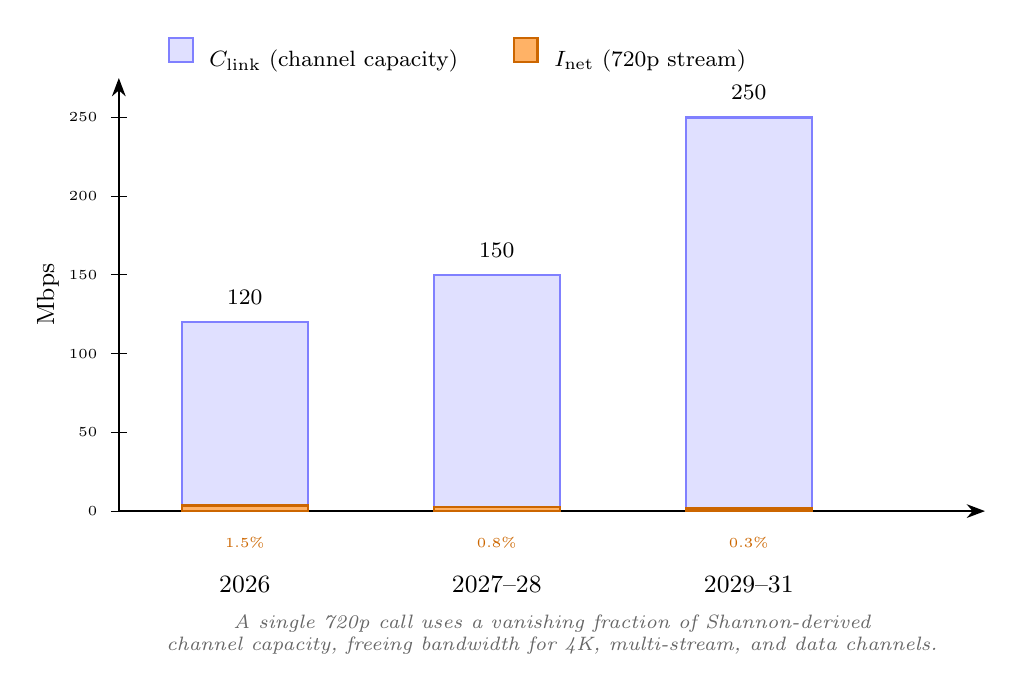
\begin{tikzpicture}[>=Stealth]

% --- Axes ---
\draw[->, thick] (0, 0) -- (11, 0);
\draw[->, thick] (0, 0) -- (0, 5.5);

% --- Axis title ---
\node[font=\small, rotate=90] at (-0.9, 2.75) {Mbps};

% --- Y-axis labels ---
\foreach \y/\lab in {0/0, 1/50, 2/100, 3/150, 4/200, 5/250} {
  \draw (-0.1, \y) -- (0.1, \y);
  \node[font=\tiny, anchor=east] at (-0.15, \y) {\lab};
}

% --- Group: March 2026 ---
% C_link = 120 Mbps -> y = 2.4
\fill[blue!12] (0.8, 0) rectangle (2.4, 2.4);
\draw[blue!50, thick] (0.8, 0) rectangle (2.4, 2.4);
% I_net = 1.75 Mbps (midpoint) -> y = 0.035
\fill[orange!60] (0.8, 0) rectangle (2.4, 0.07);
\draw[orange!80!black, thick] (0.8, 0) rectangle (2.4, 0.07);
\node[font=\footnotesize, anchor=south] at (1.6, 2.5) {120};
\node[font=\tiny, orange!80!black] at (1.6, -0.4) {1.5\%};
\node[font=\small, anchor=north] at (1.6, -0.7) {2026};

% --- Group: 2027--2028 ---
% C_link = 150 Mbps -> y = 3.0
\fill[blue!12] (4.0, 0) rectangle (5.6, 3.0);
\draw[blue!50, thick] (4.0, 0) rectangle (5.6, 3.0);
% I_net = 1.25 Mbps (midpoint) -> y = 0.025
\fill[orange!60] (4.0, 0) rectangle (5.6, 0.05);
\draw[orange!80!black, thick] (4.0, 0) rectangle (5.6, 0.05);
\node[font=\footnotesize, anchor=south] at (4.8, 3.1) {150};
\node[font=\tiny, orange!80!black] at (4.8, -0.4) {0.8\%};
\node[font=\small, anchor=north] at (4.8, -0.7) {2027--28};

% --- Group: 2029--2031 ---
% C_link = 250 Mbps -> y = 5.0
\fill[blue!12] (7.2, 0) rectangle (8.8, 5.0);
\draw[blue!50, thick] (7.2, 0) rectangle (8.8, 5.0);
% I_net = 0.85 Mbps (midpoint) -> y = 0.017
\fill[orange!60] (7.2, 0) rectangle (8.8, 0.034);
\draw[orange!80!black, thick] (7.2, 0) rectangle (8.8, 0.034);
\node[font=\footnotesize, anchor=south] at (8.0, 5.1) {250};
\node[font=\tiny, orange!80!black] at (8.0, -0.4) {0.3\%};
\node[font=\small, anchor=north] at (8.0, -0.7) {2029--31};

% --- Legend ---
\node[anchor=west, font=\footnotesize] at (0.5, 5.8) {%
  \tikz[baseline=-0.5ex]{\fill[blue!12] (0,0) rectangle (0.3,0.3);
    \draw[blue!50, thick] (0,0) rectangle (0.3,0.3);}
  ~$C_{\text{link}}$ (channel capacity) \qquad
  \tikz[baseline=-0.5ex]{\fill[orange!60] (0,0) rectangle (0.3,0.3);
    \draw[orange!80!black, thick] (0,0) rectangle (0.3,0.3);}
  ~$I_{\text{net}}$ (720p stream)};

% --- Annotation ---
\node[font=\scriptsize\itshape, text=black!60, align=center,
  anchor=north] at (5.5, -1.2)
  {A single 720p call uses a vanishing fraction of Shannon-derived\\
   channel capacity, freeing bandwidth for 4K, multi-stream, and data channels.};

\end{tikzpicture}
\caption{Channel capacity $C_{\text{link}}$ vs.\ effective information rate
  $I_{\text{net}}$ for a single 720p/30fps stream across time horizons. The
  orange bar (stream rate) is barely visible against the blue bar (capacity),
  illustrating the growing surplus as codecs improve and bandwidth increases.}
\label{fig:inet-capacity}
\end{figure}

\subsection{Security Entropy and Key Space}

The DTLS-SRTP security architecture (RFCs~8827, 3711) protects all
WebRTC media. Information-theoretic security requires that the key
entropy exceed the information content of the protected material.

For a DTLS~1.3 handshake with ECDHE on P-256, the key agreement
provides:
\begin{equation}
  H_{\text{key}} = 128 \text{~bits of security}
  \label{eq:key-entropy}
\end{equation}

The SRTP master key is 128 bits (AES-128-GCM), giving an exhaustive
search cost of $2^{128}$ operations. The total information content of a
one-hour 720p video call at 2~Mbps is:
\begin{equation}
  I_{\text{call}} = 2 \times 10^6 \times 3600
    = 7.2 \times 10^9 \text{~bits}
    \approx 2^{32.7} \text{~bits}
  \label{eq:call-content}
\end{equation}

The ratio of key entropy to protected content:
\begin{equation}
  \frac{H_{\text{key}}}{I_{\text{call}}}
    = \frac{128}{32.7} \approx 3.91
  \label{eq:security-margin}
\end{equation}

This ratio remains comfortably above~1 even for much longer sessions.
For a continuous 24-hour 4K AV1 stream at 15~Mbps:
\begin{equation}
  I_{\text{stream}} = 15 \times 10^6 \times 86400
    = 1.296 \times 10^{12} \text{~bits}
    \approx 2^{40.2} \text{~bits}
\end{equation}
yielding $H_{\text{key}} / I_{\text{stream}} \approx 3.18$, still
well above the threshold.

\subsubsection{End-to-End Encryption via Encoded Transforms}

The RTCRtpScriptTransform API (Encoded Transforms) enables
application-layer E2EE within the WebRTC pipeline. From an
information-theoretic perspective, this introduces a second encryption
layer with its own key, creating a \emph{nested channel}:
\begin{equation}
  X \xrightarrow{\;K_{\text{E2EE}}\;}
  E_1(X) \xrightarrow{\;K_{\text{SRTP}}\;}
  E_2(E_1(X))
  \label{eq:nested}
\end{equation}

The mutual information between the ciphertext and plaintext, given
neither key, satisfies:
\begin{equation}
  I\!\left(X;\, E_2(E_1(X))\right) \leq
    \min\!\big(H(K_{\text{E2EE}})^{-1},\;
    H(K_{\text{SRTP}})^{-1}\big)
    \cdot I_{\text{call}}
  \label{eq:mutual-e2ee}
\end{equation}

In practice, with $H(K_{\text{E2EE}}) = H(K_{\text{SRTP}}) = 128$
bits, this quantity is negligible ($\ll 1$ bit for any practical
session length), confirming that the nested encryption provides
information-theoretic confidentiality well beyond computational
security guarantees.

Today (March~2026), Encoded Transforms remain Chrome-only. By
2027--2028 (Section~8.3), cross-browser standardization will make
this nested channel universally available. By 2029--2031, SFrame
for group calls will extend this to $n$-party sessions, where the
mutual information between any non-member and the group plaintext
remains negligible:
\begin{equation}
  I\!\left(X;\, E(X) \;\middle|\; K_i \notin
    \{K_1, \ldots, K_n\}\right) \approx 0
  \label{eq:sframe}
\end{equation}

\subsection{WebTransport: Unreliable Datagrams and Channel Capacity}

WebTransport (RFC~9297) introduces unreliable datagrams to browser-server
communication. For latency-sensitive applications (game state, sensor
telemetry), the relevant measure is not throughput but
\emph{freshness-weighted information rate}. Define the value of a
datagram as exponentially decaying with delivery latency $\delta$:
\begin{equation}
  V(\delta) = e^{-\lambda \delta}
  \label{eq:freshness}
\end{equation}
where $\lambda > 0$ is an application-specific decay rate. The
effective information rate under unreliable delivery is:
\begin{equation}
  I_{\text{WT}} = R_{\text{send}} \cdot (1 - p_{\text{loss}})
    \cdot \mathbb{E}\!\left[e^{-\lambda \delta}\right]
  \label{eq:iwt}
\end{equation}

Under reliable delivery (TCP/WebSocket), a retransmission delays
subsequent data, so:
\begin{equation}
  I_{\text{WS}} = R_{\text{send}}
    \cdot \mathbb{E}\!\left[e^{-\lambda(\delta + p \cdot 2\tau)}\right]
  \label{eq:iws}
\end{equation}

The ratio $I_{\text{WT}} / I_{\text{WS}}$ exceeds 1 when:
\begin{equation}
  (1 - p) \cdot e^{\lambda \cdot p \cdot 2\tau} > 1
  \quad \Longleftrightarrow \quad
  \lambda > \frac{-\ln(1 - p)}{2 p \tau}
  \label{eq:wt-advantage}
\end{equation}

For $p = 0.02$ and $\tau = 25$~ms, this gives $\lambda > 20.2$~s$^{-1}$
(half-life $< 34$~ms).

\excursus{Excursus: Why $p = 0.02$ and $\tau = 25$\,ms?}{These values represent
median fixed-broadband conditions in 2026 (Table~\ref{tab:inet}). On mobile or
congested links ($p \approx 0.05$, $\tau \approx 50$\,ms), the threshold
$\lambda^*$ drops to ${\sim}10$\,s$^{-1}$, broadening WebTransport's advantage
to applications with data half-lives up to ${\sim}70$\,ms. The fixed-broadband
reference is thus conservative: mobile scenarios favor unreliable delivery even
more strongly.}

Any application where data older than
$\sim$30~ms is useless benefits from WebTransport's unreliable
mode over WebSocket --- precisely the regime of interactive gaming, live
cursor tracking, and real-time sensor feeds.

As of March~2026, Safari does not support WebTransport
(Section~5), limiting coverage to $\sim$82\%. By 2027--2028
(Section~8.2), universal support will allow applications to rely on
(\ref{eq:iwt}) without fallback paths.

\begin{figure}[ht]
\centering
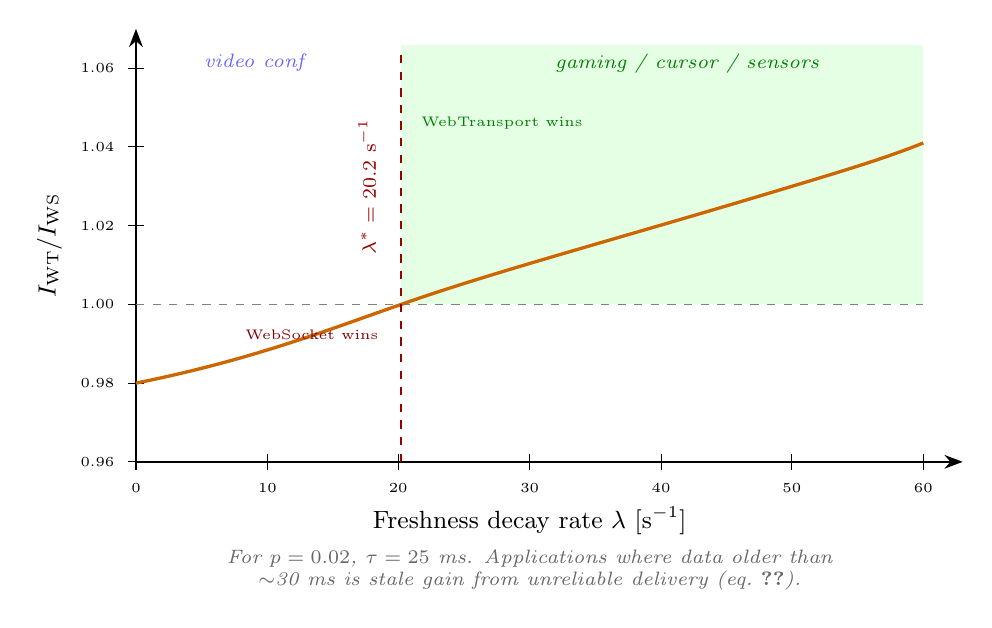
\begin{tikzpicture}[>=Stealth]

% --- Axes ---
\draw[->, thick] (0, 0) -- (10.5, 0);
\draw[->, thick] (0, 0) -- (0, 5.5);

% --- Axis titles (positioned to clear tick labels) ---
\node[font=\small] at (5, -0.75)
  {Freshness decay rate $\lambda$ [s$^{-1}$]};
\node[font=\small, rotate=90] at (-1.1, 2.75)
  {$I_{\text{WT}} / I_{\text{WS}}$};

% --- X-axis labels ---
\foreach \x/\lab in {0/0, 1.67/10, 3.33/20, 5.0/30, 6.67/40, 8.33/50, 10/60} {
  \draw (\x, -0.1) -- (\x, 0.1);
  \node[font=\tiny, anchor=north] at (\x, -0.15) {\lab};
}

% --- Y-axis labels (0.96 to 1.06, each 0.02 = 1 unit) ---
\foreach \y/\lab in {0/0.96, 1/0.98, 2/1.00, 3/1.02, 4/1.04, 5/1.06} {
  \draw (-0.1, \y) -- (0.1, \y);
  \node[font=\tiny, anchor=east] at (-0.15, \y) {\lab};
}

% --- Ratio = 1.0 line (y=2 maps to ratio 1.0) ---
\draw[thin, gray, dashed] (0, 2) -- (10, 2);

% --- Shade WebTransport advantage region ---
% lambda* = 20.2 -> x = 3.37
\fill[green!10] (3.37, 2) rectangle (10, 5.3);

% --- I_WT/I_WS curve: 0.98*exp(lambda*0.001) ---
% Y range: 0.96-1.06 (each 0.02 = 1 unit). lambda=0: y=1, lambda*=20.2: y=2, lambda=60: y=4.05
\draw[very thick, orange!80!black]
  (0, 1.0) .. controls (1.5, 1.3) and (2.5, 1.7) ..
  (3.37, 2.0) .. controls (4.5, 2.4) and (6, 2.8) ..
  (8, 3.4) .. controls (9, 3.7) and (9.5, 3.85) ..
  (10, 4.05);

% --- Threshold line ---
\draw[thick, dashed, red!60!black] (3.37, 0) -- (3.37, 5.2);
\node[font=\scriptsize, red!60!black, anchor=south, rotate=90] at (3.17, 3.5)
  {$\lambda^* = 20.2$ s$^{-1}$};

% --- Application regime labels ---
\node[font=\scriptsize\itshape, text=blue!60, anchor=north] at (1.5, 5.3)
  {video conf};
\node[font=\scriptsize\itshape, text=green!50!black, anchor=north] at (7.0, 5.3)
  {gaming / cursor / sensors};

% --- Mark advantage/disadvantage ---
\node[font=\tiny, text=red!50!black, anchor=north east] at (3.2, 1.8)
  {WebSocket wins};
\node[font=\tiny, text=green!50!black, anchor=north west] at (3.5, 4.5)
  {WebTransport wins};

% --- Annotation ---
\node[font=\scriptsize\itshape, text=black!60, align=center,
  anchor=north] at (5.0, -1.0)
  {For $p = 0.02$, $\tau = 25$~ms. Applications where data older than\\
   ${\sim}$30~ms is stale gain from unreliable delivery (eq.~\ref{eq:wt-advantage}).};

\end{tikzpicture}
\caption{Freshness-weighted information rate ratio $I_{\text{WT}} / I_{\text{WS}}$
  as a function of decay rate $\lambda$. Above the threshold $\lambda^*$,
  WebTransport's unreliable datagrams deliver more useful information per
  unit time than WebSocket's reliable delivery, because retransmission
  wastes capacity on stale data.}
\label{fig:freshness}
\end{figure}

\subsection{Projections Summary and Practical Implications}

\begin{table}[ht]
\centering
\small
\renewcommand{\arraystretch}{1.4}
\begin{tabularx}{\textwidth}{lXXX}
\toprule
\textbf{Measure} & \textbf{March 2026} & \textbf{2027--2028} &
  \textbf{2029--2031} \\
\midrule
Channel capacity $C_{\text{link}}$ &
  120~Mbps &
  150~Mbps &
  250~Mbps \\
HOL blocking factor $(1\!-\!p)^{n-2}$ at $n\!=\!8$ &
  0.94 ($p\!=\!0.01$) &
  0.94 &
  0.97 ($p\!=\!0.005$) \\
Source coding gap $\Delta$ &
  VP9: $\sim$0.8 &
  AV1 HW: $\sim$0.5 &
  AV1 opt: $\sim$0.4 \\
$I_{\text{net}}$ per 720p stream &
  1.3--2.2~Mbps &
  0.9--1.6~Mbps &
  0.6--1.1~Mbps \\
Max 720p streams in $C_{\text{link}}$ &
  $\sim$55--90 &
  $\sim$95--165 &
  $\sim$230--415 \\
E2EE availability &
  Chrome only &
  Cross-browser &
  SFrame $n$-party \\
WebTransport coverage &
  82\% &
  $\sim$100\% &
  100\% \\
Freshness threshold $\lambda^*$ &
  20.2~s$^{-1}$ &
  $\sim$18~s$^{-1}$ &
  $\sim$15~s$^{-1}$ \\
\bottomrule
\end{tabularx}
\caption{Information-theoretic measures across time horizons. $\Delta$
  is the coding efficiency gap (\ref{eq:coding-gap}), $I_{\text{net}}$
  is the net information rate (\ref{eq:inet}), and $\lambda^*$ is the
  freshness decay threshold above which WebTransport dominates WebSocket
  (\ref{eq:wt-advantage}).}
\label{tab:projections}
\end{table}

The trajectory is clear: the combination of improving source coding
(AV1 hardware), expanding channel capacity (broadband growth), and
maturing transport protocols (QUIC universal, WebTransport universal)
drives the \emph{information cost per unit of communicated experience}
steadily downward. The remaining question is not whether the
Shannon capacity suffices --- it already does, by orders of magnitude
--- but how efficiently the protocol stack converts that capacity into
delivered, fresh, secure information at the application layer. By
2030, the gap between theoretical capacity and realized throughput will
be the narrowest it has ever been for browser-based real-time
communication.

\subsubsection{What the Theory Means for Applications}

The equations and figures in this appendix are not purely academic. Each
theoretical result maps to a concrete design decision that application
developers face today and over the next five years.

\textbf{Codec selection determines bandwidth cost, not quality.}
The rate-distortion analysis (Section~A.2, Figure~\ref{fig:rate-distortion})
shows that AV1 operates at roughly 46\% of H.264's bit rate for equivalent
perceptual quality at 720p. In practice, this means a WebRTC application
switching from H.264 to AV1 can either halve its bandwidth consumption at
the same quality or substantially increase resolution (e.g., 720p to 1080p)
within the same bandwidth envelope. By 2030, with AV1 hardware encoding
ubiquitous and the coding gap $\Delta$ approaching 0.4, further codec
improvements yield diminishing returns --- the stack will be operating close
enough to the Shannon rate-distortion bound that the next generation of
efficiency gains will come from transport and architecture, not codecs alone.

\textbf{QUIC's advantage is situational but decisive on bad networks.}
The head-of-line blocking analysis (Section~A.1.1,
Figure~\ref{fig:hol-blocking}) shows that QUIC's per-stream throughput
advantage over TCP is modest on good networks (6\% at 1\% loss) but
substantial on degraded ones (34\% at 5\% loss). The practical implication
is that applications targeting mobile users, emerging markets, or congested
enterprise networks --- precisely the environments where real-time
communication is hardest --- benefit disproportionately from QUIC-based
transports. For a video conference with 8 participants on a cellular
connection experiencing 3--5\% packet loss, the difference between QUIC and
TCP is the difference between usable and degraded video.

\textbf{Connection latency is a solved problem for returning users.}
The handshake analysis (Section~A.1.2) shows that QUIC 0-RTT eliminates
connection establishment overhead entirely for resumed connections. For a
WebTransport application that a user opens daily --- a collaboration tool,
a live dashboard, a recurring meeting client --- the time to first useful
byte drops to zero. The 1.125~MB of wasted capacity during a TCP+TLS
handshake on a 120~Mbps link may seem small, but for latency-sensitive
applications where the first 100~ms of perceived responsiveness determines
user experience, the difference is measurable.

\textbf{Bandwidth surplus enables architectural ambition.}
The effective information rate analysis (Section~A.3,
Figure~\ref{fig:inet-capacity}) reveals the most consequential practical
finding: a single 720p video stream consumes a vanishing fraction of
available link capacity (under 0.5\% by 2030). This surplus is not merely
``headroom'' --- it is the resource that makes new application architectures
feasible. A 250~Mbps link can theoretically carry 230--415 simultaneous 720p
streams. In practice, this means applications can afford to run multiple
concurrent media flows (video, screen share, spatial audio), data channels
(collaborative editing, file transfer), and telemetry streams without
contending for bandwidth. The constraint shifts from ``can the network carry
this?''\ to ``can the application manage this complexity?''

\textbf{End-to-end encryption adds negligible overhead.}
The security analysis (Section~A.4) confirms that the nested DTLS-SRTP plus
E2EE architecture imposes no meaningful information-theoretic cost. The key
entropy ($2^{128}$) exceeds the information content of any practical session
by a factor of at least 3. For application developers, this means E2EE can
be treated as a default rather than a premium feature --- there is no
bandwidth, latency, or capacity penalty for encrypting at the application
layer on top of the transport-layer encryption that WebRTC already mandates.
The only constraint is API availability, which moves from Chrome-only (2026)
to universal (2028).

\textbf{WebTransport unlocks real-time data that WebSocket cannot serve.}
The freshness analysis (Section~A.5, Figure~\ref{fig:freshness}) quantifies
when unreliable delivery outperforms reliable delivery: any data with a
useful half-life below approximately 34~ms benefits from WebTransport's
unreliable datagrams. This covers a wide class of interactive applications
--- game state synchronization, live cursor and pointer sharing, real-time
sensor feeds, collaborative whiteboard strokes --- where retransmitting a
stale update is worse than dropping it. Before WebTransport, these
applications had to choose between WebSocket (reliable but stale under loss)
and WebRTC DataChannel (unreliable mode available but requiring the full
peer-to-peer ICE/DTLS machinery). WebTransport provides the unreliable
mode with a simple client-server model over HTTP/3, removing the
architectural overhead.

\textbf{The overall picture: the stack converges on efficiency.}
Taken together, the information-theoretic measures trace a consistent
trajectory. The protocol stack is converging toward the theoretical limits
established by Shannon: codecs approach the rate-distortion bound, transports
eliminate unnecessary blocking and handshake overhead, and encryption adds
negligible cost. By 2030, the practical distance between what the standards
deliver and what information theory permits will be the smallest it has ever
been for browser-based real-time communication. The consequence for
application developers is that the infrastructure --- standards, hardware,
and networks --- will no longer be the binding constraint. The remaining
challenge is purely architectural: how to compose these efficient, universal
primitives into applications that fully exploit the capacity and low latency
they provide.

%
% Requires in the preamble: amsmath, amssymb, tabularx, booktabs

\section{Information-Theoretic View}
\label{app:info-theory}

This appendix applies information-theoretic measures to the real-time
web communication stack described in this document. We quantify channel
capacity, source coding efficiency, and effective information rates
across three time horizons: today (March~2026), the near term
(2027--2028), and the medium term (2029--2031). The analysis draws on
the standards, codec parameters, and infrastructure projections
developed in the main text.

\subsection{Channel Capacity of the Transport Layer}

The Shannon-Hartley theorem gives the theoretical maximum information
rate for a channel with additive white Gaussian noise:
\begin{equation}
  C = B \log_2\!\left(1 + \frac{S}{N}\right) \quad \text{[bits/s]}
  \label{eq:shannon}
\end{equation}
where $B$ is the channel bandwidth in Hz and $S/N$ is the
signal-to-noise ratio.

While the physical-layer capacity of a broadband link is governed by
(\ref{eq:shannon}), the \emph{effective} capacity available to the
application is reduced by protocol overhead, congestion control, and
transport inefficiencies. We define the effective application-layer
throughput as:
\begin{equation}
  R_{\text{eff}} = C_{\text{link}} \cdot \eta_{\text{transport}}
    \cdot (1 - \rho_{\text{overhead}})
  \label{eq:reff}
\end{equation}
where $C_{\text{link}}$ is the link-layer capacity,
$\eta_{\text{transport}} \in (0,1]$ is the transport efficiency factor
(capturing congestion control, retransmission, and multiplexing
behavior), and $\rho_{\text{overhead}} \in [0,1)$ is the fractional
protocol overhead (headers, encryption, framing).

\subsubsection{Head-of-Line Blocking and Multiplexed Capacity}

Consider $n$ independent streams multiplexed over a single connection.
Under TCP (HTTP/2), a single lost packet blocks all $n$ streams. The
expected throughput per stream under loss rate $p$ is bounded by:
\begin{equation}
  R_{\text{TCP}}^{(i)} \leq \frac{R_{\text{eff}}}{n}
    \cdot (1 - p)^{n-1}
  \label{eq:hol-tcp}
\end{equation}
because a loss in \emph{any} of the $n$ streams stalls all others. Under
QUIC (RFC~9000), streams are independent at the transport layer, so:
\begin{equation}
  R_{\text{QUIC}}^{(i)} \leq \frac{R_{\text{eff}}}{n}
    \cdot (1 - p)
  \label{eq:hol-quic}
\end{equation}
The ratio of effective per-stream throughput is:
\begin{equation}
  \frac{R_{\text{QUIC}}^{(i)}}{R_{\text{TCP}}^{(i)}}
    = \frac{1}{(1-p)^{n-2}}
  \label{eq:hol-ratio}
\end{equation}
\excursus{Excursus: Why $n = 8$?}{In a typical multi-participant video
conference, each peer contributes multiple concurrent streams: a camera video
track, an audio track, and often a screen-share or data channel. A four-person
call with two media tracks each produces $n = 8$ multiplexed streams over a
single connection --- the reference value used throughout this section. Larger
meetings (e.g.\ 10 participants with simulcast layers) push $n$ higher,
amplifying the HOL blocking effect further.}

For $n = 8$ streams (a typical multi-track video conference) at
$p = 0.01$ (1\% loss), this gives a QUIC advantage factor of
$1/(0.99)^6 \approx 1.062$, a modest 6.2\% improvement. At $p = 0.05$
(5\% loss, common on mobile or congested links), the factor is
$1/(0.95)^6 \approx 1.34$, a 34\% throughput advantage per stream.

\begin{figure}[ht]
\centering
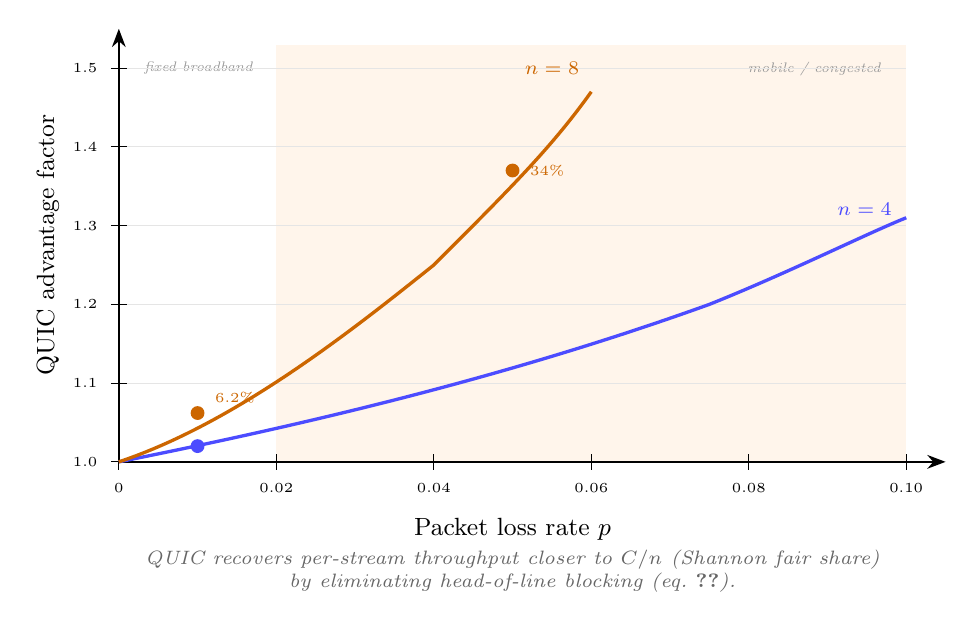
\begin{tikzpicture}[>=Stealth]

% --- Shaded region (drawn FIRST so curves appear on top) ---
\fill[orange!8] (2, 0) rectangle (10, 5.3);
\node[font=\tiny\itshape, text=black!40, anchor=north east] at (9.8, 5.2)
  {mobile / congested};
\node[font=\tiny\itshape, text=black!40, anchor=north west] at (0.2, 5.2)
  {fixed broadband};

% --- Grid lines ---
\foreach \y in {1, 2, 3, 4, 5} {
  \draw[gray!20] (0, \y) -- (10, \y);
}

% --- Axes ---
\draw[->, thick] (0, 0) -- (10.5, 0);
\draw[->, thick] (0, 0) -- (0, 5.5);

% --- Axis titles (positioned to clear tick labels) ---
\node[font=\small] at (5, -0.85) {Packet loss rate $p$};
\node[font=\small, rotate=90] at (-0.9, 2.75) {QUIC advantage factor};

% --- X-axis labels ---
\foreach \x/\lab in {0/0, 2/0.02, 4/0.04, 6/0.06, 8/0.08, 10/0.10} {
  \draw (\x, -0.1) -- (\x, 0.1);
  \node[font=\tiny, anchor=north] at (\x, -0.15) {\lab};
}

% --- Y-axis labels ---
\foreach \y/\lab in {0/1.0, 1/1.1, 2/1.2, 3/1.3, 4/1.4, 5/1.5} {
  \draw (-0.1, \y) -- (0.1, \y);
  \node[font=\tiny, anchor=east] at (-0.15, \y) {\lab};
}

% --- n=4 curve: 1/(1-p)^2 ---
\draw[very thick, blue!70]
  (0, 0) .. controls (2.5, 0.5) and (5, 1.1) ..
  (7.5, 2.0) .. controls (8.5, 2.4) and (9.5, 2.9) ..
  (10, 3.1);
\node[font=\scriptsize, blue!70, anchor=south west] at (9.0, 3.0)
  {$n = 4$};

% --- n=8 curve: 1/(1-p)^6 ---
\draw[very thick, orange!80!black]
  (0, 0) .. controls (1.5, 0.5) and (3, 1.7) ..
  (4, 2.5) .. controls (5, 3.5) and (5.5, 4.0) ..
  (6, 4.7);
\node[font=\scriptsize, orange!80!black, anchor=south] at (5.5, 4.8)
  {$n = 8$};

% --- Reference points ---
\fill[orange!80!black] (1.0, 0.62) circle (2.5pt);
\node[font=\tiny, orange!80!black, anchor=south west] at (1.1, 0.62)
  {6.2\%};

\fill[orange!80!black] (5.0, 3.7) circle (2.5pt);
\node[font=\tiny, orange!80!black, anchor=west] at (5.1, 3.7)
  {34\%};

\fill[blue!70] (1.0, 0.20) circle (2.5pt);

% --- Annotation ---
\node[font=\scriptsize\itshape, text=black!60, align=center,
  anchor=north] at (5.0, -1.0)
  {QUIC recovers per-stream throughput closer to $C/n$ (Shannon fair share)\\
   by eliminating head-of-line blocking (eq.~\ref{eq:hol-ratio}).};

\end{tikzpicture}
\caption{QUIC advantage factor $1/(1-p)^{n-2}$ over TCP for multiplexed
  streams. At 5\% loss with $n=8$ streams, QUIC delivers 34\% more
  per-stream throughput by maintaining independence at the transport layer.}
\label{fig:hol-blocking}
\end{figure}

\subsubsection{Connection Establishment Latency}

Let $\tau$ denote the one-way latency (half the round-trip time). The
information-carrying capacity during connection establishment is zero;
the handshake represents pure overhead. The time to first useful byte
is:
\begin{align}
  T_{\text{TCP+TLS\,1.3}} &= 2\tau_{\text{TCP}} + \tau_{\text{TLS}}
    = 3\tau \quad \text{(1-RTT TLS~1.3)} \label{eq:tcp-setup} \\
  T_{\text{QUIC}} &= \tau \quad \text{(1-RTT)}
    \label{eq:quic-setup} \\
  T_{\text{QUIC,\,0-RTT}} &= 0 \quad \text{(resumption)}
    \label{eq:quic-0rtt}
\end{align}
The QUIC 0-RTT case (\ref{eq:quic-0rtt}) eliminates the handshake
entirely for resumed connections. The information lost during
handshake dead time, relative to steady-state capacity, is:
\begin{equation}
  I_{\text{lost}} = C_{\text{link}} \cdot T_{\text{setup}}
  \label{eq:ilost}
\end{equation}
For a 120~Mbps link with $\tau = 25$~ms (typical fixed broadband in
2026), the TCP+TLS~1.3 handshake wastes $120 \times 10^6 \times 0.075
= 9 \times 10^6$ bits (1.125~MB), while QUIC~1-RTT wastes only
$3 \times 10^6$ bits (375~KB).

\subsection{Source Coding Efficiency}

The rate-distortion function $R(D)$ defines the minimum bit rate
required to represent a source at distortion level $D$. For a
Gaussian source with variance $\sigma^2$ under mean squared error
distortion:
\begin{equation}
  R(D) = \frac{1}{2} \log_2 \frac{\sigma^2}{D}
    \quad \text{[bits/sample]}
  \label{eq:rate-distortion}
\end{equation}

\excursus{Excursus: Why Gaussian source?}{The Gaussian memoryless model is used
because it yields the highest (worst-case) $R(D)$ among all sources of equal
variance. Any codec that approaches the Gaussian bound on real video is
therefore doing at least as well as the bound predicts --- the true $R(D)$ for
spatially and temporally correlated video lies below the Gaussian curve, making
it a conservative benchmark.}

No practical codec achieves $R(D)$;\footnote{The $R(D)$ curve in
Figure~\ref{fig:rate-distortion} is the Gaussian memoryless source bound
(equation~\ref{eq:rate-distortion}), which is an upper bound on the true
$R(D)$ for non-Gaussian sources such as video.  Additionally, $R(D)$ assumes
zero excess-distortion probability, whereas practical codecs permit a
frame-level excess-distortion probability on the order of $10^{-6}$ to
$10^{-8}$.  Both factors allow codec operating points measured on real content
to approach or marginally cross the Gaussian bound.} real codecs operate at
some rate $R_{\text{codec}} > R(D)$. We define the coding efficiency gap as:
\begin{equation}
  \Delta = \frac{R_{\text{codec}} - R(D)}{R(D)}
  \label{eq:coding-gap}
\end{equation}

The codecs in the WebRTC stack can be ordered by their empirical
proximity to $R(D)$ for typical video content at conversational
resolutions (720p, 30~fps). Using published Bj\o ntegaard Delta (BD)
rate measurements:
\begin{equation}
  R_{\text{H.264}} > R_{\text{VP9}} > R_{\text{AV1}}
    > R(D)
  \label{eq:codec-ordering}
\end{equation}

Specifically, the empirical rate savings at equivalent PSNR are
approximately:
\begin{align}
  R_{\text{VP9}}  &\approx 0.65 \cdot R_{\text{H.264}}
    \quad (\sim\!35\% \text{ savings}) \label{eq:vp9-savings} \\
  R_{\text{AV1}}  &\approx 0.70 \cdot R_{\text{VP9}}
    \approx 0.46 \cdot R_{\text{H.264}}
    \quad (\sim\!30\% \text{ over VP9})
  \label{eq:av1-savings}
\end{align}

\begin{figure}[ht]
\centering
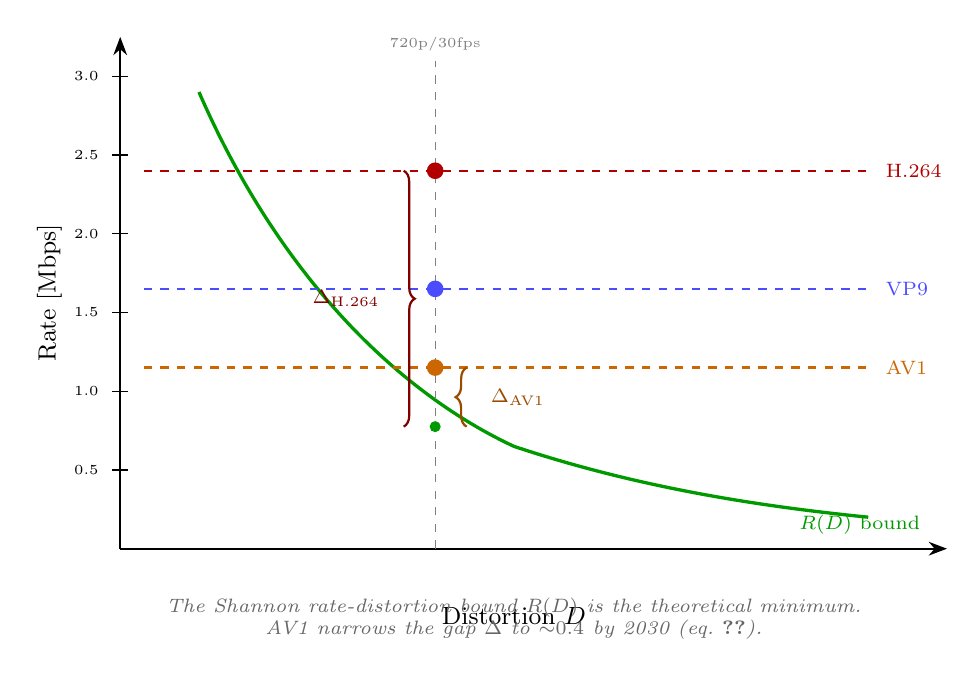
\begin{tikzpicture}[>=Stealth]

% --- Axes ---
\draw[->, thick] (0, 0) -- (10.5, 0);
\draw[->, thick] (0, 0) -- (0, 6.5);

% --- Axis titles ---
\node[font=\small] at (5, -0.85) {Distortion $D$};
\node[font=\small, rotate=90] at (-0.9, 3.25) {Rate [Mbps]};

% --- Y-axis rate labels ---
\foreach \y/\lab in {1.0/0.5, 2.0/1.0, 3.0/1.5, 4.0/2.0, 5.0/2.5, 6.0/3.0} {
  \draw (-0.1, \y) -- (0.1, \y);
  \node[font=\tiny, anchor=east] at (-0.15, \y) {\lab};
}

% --- R(D) Shannon bound curve ---
\draw[very thick, green!60!black]
  (1.0, 5.8) .. controls (2.0, 3.5) and (3.5, 2.0) ..
  (5.0, 1.3) .. controls (6.5, 0.8) and (8.0, 0.55) ..
  (9.5, 0.4);
\node[font=\scriptsize, green!60!black, anchor=north west] at (8.5, 0.55)
  {$R(D)$ bound};

% --- Reference distortion line (720p/30fps operating point) ---
\draw[thin, gray, dashed] (4.0, 0) -- (4.0, 6.2);
\node[font=\tiny, gray, anchor=south] at (4.0, 6.2) {720p/30fps};

% --- R(D) value at reference distortion ---
\fill[green!60!black] (4.0, 1.55) circle (2pt);

% --- Codec operating points at reference distortion ---
% H.264: ~2.5 Mbps
\draw[thick, dashed, red!70!black] (0.3, 4.8) -- (9.5, 4.8);
\fill[red!70!black] (4.0, 4.8) circle (3pt);
\node[font=\scriptsize, red!70!black, anchor=west] at (9.6, 4.8) {H.264};

% VP9: ~1.6 Mbps (0.65 * H.264)
\draw[thick, dashed, blue!70] (0.3, 3.3) -- (9.5, 3.3);
\fill[blue!70] (4.0, 3.3) circle (3pt);
\node[font=\scriptsize, blue!70, anchor=west] at (9.6, 3.3) {VP9};

% AV1: ~1.15 Mbps (0.46 * H.264)
\draw[thick, dashed, orange!80!black] (0.3, 2.3) -- (9.5, 2.3);
\fill[orange!80!black] (4.0, 2.3) circle (3pt);
\node[font=\scriptsize, orange!80!black, anchor=west] at (9.6, 2.3) {AV1};

% --- Gap annotations (braces) ---
% H.264 gap
\draw[decorate, decoration={brace, amplitude=4pt, mirror},
  thick, red!50!black]
  (3.6, 1.55) -- (3.6, 4.8)
  node[midway, anchor=east, font=\scriptsize, xshift=-5pt]
  {$\Delta_{\text{H.264}}$};

% AV1 gap
\draw[decorate, decoration={brace, amplitude=4pt},
  thick, orange!60!black]
  (4.4, 1.55) -- (4.4, 2.3)
  node[midway, anchor=west, font=\scriptsize, xshift=5pt]
  {$\Delta_{\text{AV1}}$};

% --- Annotation ---
\node[font=\scriptsize\itshape, text=black!60, align=center,
  anchor=north] at (5.0, -0.5)
  {The Shannon rate-distortion bound $R(D)$ is the theoretical minimum.\\
   AV1 narrows the gap $\Delta$ to ${\sim}0.4$ by 2030 (eq.~\ref{eq:coding-gap}).};

\end{tikzpicture}
\caption{Codec operating rates vs.\ the Shannon rate-distortion bound $R(D)$
  at 720p/30fps. Each codec operates above the theoretical minimum; the gap
  $\Delta$ (eq.~\ref{eq:coding-gap}) shrinks from H.264 through VP9 to AV1,
  approaching but never reaching the bound.}
\label{fig:rate-distortion}
\end{figure}

\subsubsection{Codec Entropy and WebCodecs}

The WebCodecs API (W3C Working Draft) exposes per-frame codec access,
allowing measurement and control of the instantaneous encoding rate.
For a video frame $f_t$ at time $t$, the encoder output has empirical
entropy:
\begin{equation}
  \hat{H}(f_t) = -\sum_{s \in \mathcal{S}}
    p(s \mid f_t) \log_2 p(s \mid f_t)
  \label{eq:frame-entropy}
\end{equation}
where $\mathcal{S}$ is the set of symbols emitted by the entropy coder
(CABAC for H.264/AV1, arithmetic coding for VP9). WebCodecs enables
applications to observe $|E(f_t)|$ (the encoded frame size in bits)
directly, which serves as a practical upper bound on
$\hat{H}(f_t)$:
\begin{equation}
  \hat{H}(f_t) \leq |E(f_t)| \leq R_{\text{codec}} / \text{fps}
  \label{eq:entropy-bound}
\end{equation}

\subsection{Effective Information Rate by Time Horizon}

We now combine transport and source coding measures to estimate the
effective information rate for a representative real-time video
session: a single 720p/30fps video call with one audio channel.

\excursus{Excursus: Why 720p?}{Throughout this appendix, 720p/30fps is used as
a fixed reference for cross-era comparison, not as a prediction that 720p
remains the dominant conferencing resolution. The bandwidth surplus quantified
below is precisely what enables migration to 1080p (feasible by ${\sim}$2028
with AV1 hardware encode at today's 720p bit rates) and 4K (feasible by
${\sim}$2030). The 720p baseline makes the efficiency gains legible: the same
task gets cheaper, freeing capacity for higher quality or more streams.}

Define the \emph{net information rate} as:
\begin{equation}
  I_{\text{net}} = R_{\text{codec}} \cdot \eta_{\text{transport}}
    \cdot (1 - \rho_{\text{overhead}})
    \cdot (1 - p_{\text{loss}})
  \label{eq:inet}
\end{equation}

\begin{table}[ht]
\centering
\small
\renewcommand{\arraystretch}{1.4}
\begin{tabularx}{\textwidth}{lXXX}
\toprule
\textbf{Parameter} & \textbf{March 2026} & \textbf{2027--2028} &
  \textbf{2029--2031} \\
\midrule
Median link capacity &
  120~Mbps &
  $\sim$150~Mbps &
  200--300~Mbps \\
Dominant codec (WebRTC) &
  VP9 / H.264 &
  VP9 / AV1 (HW) &
  AV1 (HW default) \\
Codec rate (720p/30fps) &
  1.5--2.5~Mbps &
  1.0--1.8~Mbps &
  0.7--1.2~Mbps \\
$\eta_{\text{transport}}$ &
  0.92 (QUIC) &
  0.93 &
  0.94 \\
$\rho_{\text{overhead}}$ (SRTP+QUIC) &
  0.06 &
  0.05 &
  0.04 \\
Typical loss $p$ &
  0.01--0.03 &
  0.01--0.02 &
  0.005--0.01 \\
$I_{\text{net}}$ (720p video) &
  1.3--2.2~Mbps &
  0.9--1.6~Mbps &
  0.6--1.1~Mbps \\
$I_{\text{net}}$ as \% of $C_{\text{link}}$ &
  1.1--1.8\% &
  0.6--1.1\% &
  0.2--0.6\% \\
\bottomrule
\end{tabularx}
\caption{Effective information rate for a 720p/30fps WebRTC video stream.
  The declining ratio $I_{\text{net}} / C_{\text{link}}$ reflects both
  improved codec efficiency and growing link capacity, freeing bandwidth
  for higher resolutions, additional streams, or concurrent data
  channels.}
\label{tab:inet}
\end{table}

The declining ratio $I_{\text{net}} / C_{\text{link}}$ in
Table~\ref{tab:inet} is the central quantitative observation: by 2030, a
720p video call consumes less than 0.5\% of available link capacity. The
surplus capacity enables qualitative changes --- 4K video conferencing,
multi-stream layouts, or concurrent data channels via WebTransport ---
that are quantitatively infeasible in 2026.

\begin{figure}[ht]
\centering
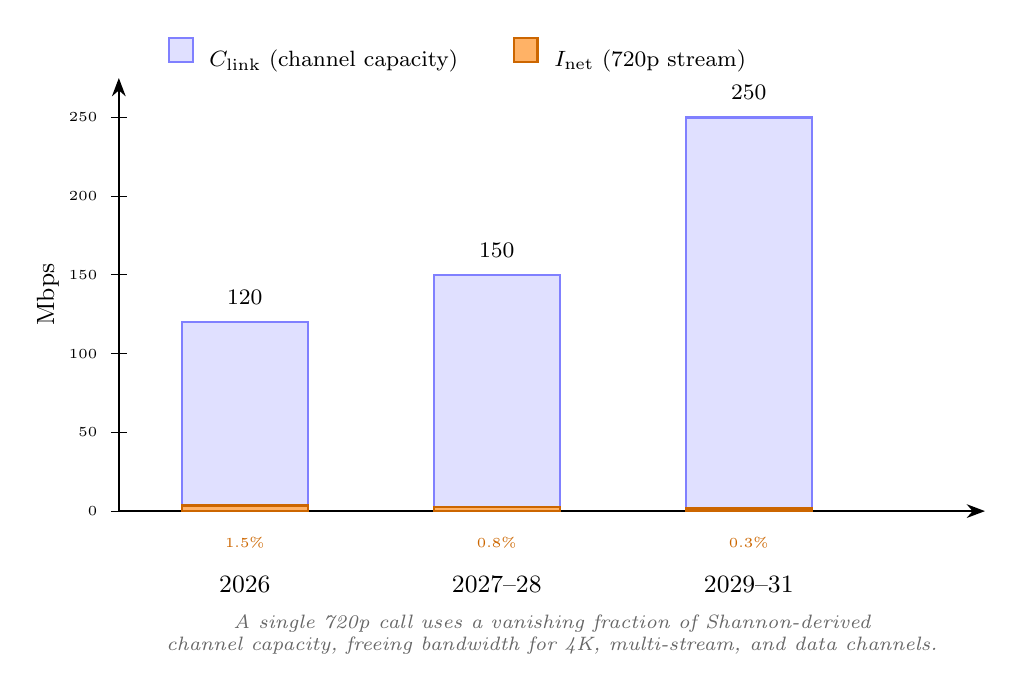
\begin{tikzpicture}[>=Stealth]

% --- Axes ---
\draw[->, thick] (0, 0) -- (11, 0);
\draw[->, thick] (0, 0) -- (0, 5.5);

% --- Axis title ---
\node[font=\small, rotate=90] at (-0.9, 2.75) {Mbps};

% --- Y-axis labels ---
\foreach \y/\lab in {0/0, 1/50, 2/100, 3/150, 4/200, 5/250} {
  \draw (-0.1, \y) -- (0.1, \y);
  \node[font=\tiny, anchor=east] at (-0.15, \y) {\lab};
}

% --- Group: March 2026 ---
% C_link = 120 Mbps -> y = 2.4
\fill[blue!12] (0.8, 0) rectangle (2.4, 2.4);
\draw[blue!50, thick] (0.8, 0) rectangle (2.4, 2.4);
% I_net = 1.75 Mbps (midpoint) -> y = 0.035
\fill[orange!60] (0.8, 0) rectangle (2.4, 0.07);
\draw[orange!80!black, thick] (0.8, 0) rectangle (2.4, 0.07);
\node[font=\footnotesize, anchor=south] at (1.6, 2.5) {120};
\node[font=\tiny, orange!80!black] at (1.6, -0.4) {1.5\%};
\node[font=\small, anchor=north] at (1.6, -0.7) {2026};

% --- Group: 2027--2028 ---
% C_link = 150 Mbps -> y = 3.0
\fill[blue!12] (4.0, 0) rectangle (5.6, 3.0);
\draw[blue!50, thick] (4.0, 0) rectangle (5.6, 3.0);
% I_net = 1.25 Mbps (midpoint) -> y = 0.025
\fill[orange!60] (4.0, 0) rectangle (5.6, 0.05);
\draw[orange!80!black, thick] (4.0, 0) rectangle (5.6, 0.05);
\node[font=\footnotesize, anchor=south] at (4.8, 3.1) {150};
\node[font=\tiny, orange!80!black] at (4.8, -0.4) {0.8\%};
\node[font=\small, anchor=north] at (4.8, -0.7) {2027--28};

% --- Group: 2029--2031 ---
% C_link = 250 Mbps -> y = 5.0
\fill[blue!12] (7.2, 0) rectangle (8.8, 5.0);
\draw[blue!50, thick] (7.2, 0) rectangle (8.8, 5.0);
% I_net = 0.85 Mbps (midpoint) -> y = 0.017
\fill[orange!60] (7.2, 0) rectangle (8.8, 0.034);
\draw[orange!80!black, thick] (7.2, 0) rectangle (8.8, 0.034);
\node[font=\footnotesize, anchor=south] at (8.0, 5.1) {250};
\node[font=\tiny, orange!80!black] at (8.0, -0.4) {0.3\%};
\node[font=\small, anchor=north] at (8.0, -0.7) {2029--31};

% --- Legend ---
\node[anchor=west, font=\footnotesize] at (0.5, 5.8) {%
  \tikz[baseline=-0.5ex]{\fill[blue!12] (0,0) rectangle (0.3,0.3);
    \draw[blue!50, thick] (0,0) rectangle (0.3,0.3);}
  ~$C_{\text{link}}$ (channel capacity) \qquad
  \tikz[baseline=-0.5ex]{\fill[orange!60] (0,0) rectangle (0.3,0.3);
    \draw[orange!80!black, thick] (0,0) rectangle (0.3,0.3);}
  ~$I_{\text{net}}$ (720p stream)};

% --- Annotation ---
\node[font=\scriptsize\itshape, text=black!60, align=center,
  anchor=north] at (5.5, -1.2)
  {A single 720p call uses a vanishing fraction of Shannon-derived\\
   channel capacity, freeing bandwidth for 4K, multi-stream, and data channels.};

\end{tikzpicture}
\caption{Channel capacity $C_{\text{link}}$ vs.\ effective information rate
  $I_{\text{net}}$ for a single 720p/30fps stream across time horizons. The
  orange bar (stream rate) is barely visible against the blue bar (capacity),
  illustrating the growing surplus as codecs improve and bandwidth increases.}
\label{fig:inet-capacity}
\end{figure}

\subsection{Security Entropy and Key Space}

The DTLS-SRTP security architecture (RFCs~8827, 3711) protects all
WebRTC media. Information-theoretic security requires that the key
entropy exceed the information content of the protected material.

For a DTLS~1.3 handshake with ECDHE on P-256, the key agreement
provides:
\begin{equation}
  H_{\text{key}} = 128 \text{~bits of security}
  \label{eq:key-entropy}
\end{equation}

The SRTP master key is 128 bits (AES-128-GCM), giving an exhaustive
search cost of $2^{128}$ operations. The total information content of a
one-hour 720p video call at 2~Mbps is:
\begin{equation}
  I_{\text{call}} = 2 \times 10^6 \times 3600
    = 7.2 \times 10^9 \text{~bits}
    \approx 2^{32.7} \text{~bits}
  \label{eq:call-content}
\end{equation}

The ratio of key entropy to protected content:
\begin{equation}
  \frac{H_{\text{key}}}{I_{\text{call}}}
    = \frac{128}{32.7} \approx 3.91
  \label{eq:security-margin}
\end{equation}

This ratio remains comfortably above~1 even for much longer sessions.
For a continuous 24-hour 4K AV1 stream at 15~Mbps:
\begin{equation}
  I_{\text{stream}} = 15 \times 10^6 \times 86400
    = 1.296 \times 10^{12} \text{~bits}
    \approx 2^{40.2} \text{~bits}
\end{equation}
yielding $H_{\text{key}} / I_{\text{stream}} \approx 3.18$, still
well above the threshold.

\subsubsection{End-to-End Encryption via Encoded Transforms}

The RTCRtpScriptTransform API (Encoded Transforms) enables
application-layer E2EE within the WebRTC pipeline. From an
information-theoretic perspective, this introduces a second encryption
layer with its own key, creating a \emph{nested channel}:
\begin{equation}
  X \xrightarrow{\;K_{\text{E2EE}}\;}
  E_1(X) \xrightarrow{\;K_{\text{SRTP}}\;}
  E_2(E_1(X))
  \label{eq:nested}
\end{equation}

The mutual information between the ciphertext and plaintext, given
neither key, satisfies:
\begin{equation}
  I\!\left(X;\, E_2(E_1(X))\right) \leq
    \min\!\big(H(K_{\text{E2EE}})^{-1},\;
    H(K_{\text{SRTP}})^{-1}\big)
    \cdot I_{\text{call}}
  \label{eq:mutual-e2ee}
\end{equation}

In practice, with $H(K_{\text{E2EE}}) = H(K_{\text{SRTP}}) = 128$
bits, this quantity is negligible ($\ll 1$ bit for any practical
session length), confirming that the nested encryption provides
information-theoretic confidentiality well beyond computational
security guarantees.

Today (March~2026), Encoded Transforms remain Chrome-only. By
2027--2028 (Section~8.3), cross-browser standardization will make
this nested channel universally available. By 2029--2031, SFrame
for group calls will extend this to $n$-party sessions, where the
mutual information between any non-member and the group plaintext
remains negligible:
\begin{equation}
  I\!\left(X;\, E(X) \;\middle|\; K_i \notin
    \{K_1, \ldots, K_n\}\right) \approx 0
  \label{eq:sframe}
\end{equation}

\subsection{WebTransport: Unreliable Datagrams and Channel Capacity}

WebTransport (RFC~9297) introduces unreliable datagrams to browser-server
communication. For latency-sensitive applications (game state, sensor
telemetry), the relevant measure is not throughput but
\emph{freshness-weighted information rate}. Define the value of a
datagram as exponentially decaying with delivery latency $\delta$:
\begin{equation}
  V(\delta) = e^{-\lambda \delta}
  \label{eq:freshness}
\end{equation}
where $\lambda > 0$ is an application-specific decay rate. The
effective information rate under unreliable delivery is:
\begin{equation}
  I_{\text{WT}} = R_{\text{send}} \cdot (1 - p_{\text{loss}})
    \cdot \mathbb{E}\!\left[e^{-\lambda \delta}\right]
  \label{eq:iwt}
\end{equation}

Under reliable delivery (TCP/WebSocket), a retransmission delays
subsequent data, so:
\begin{equation}
  I_{\text{WS}} = R_{\text{send}}
    \cdot \mathbb{E}\!\left[e^{-\lambda(\delta + p \cdot 2\tau)}\right]
  \label{eq:iws}
\end{equation}

The ratio $I_{\text{WT}} / I_{\text{WS}}$ exceeds 1 when:
\begin{equation}
  (1 - p) \cdot e^{\lambda \cdot p \cdot 2\tau} > 1
  \quad \Longleftrightarrow \quad
  \lambda > \frac{-\ln(1 - p)}{2 p \tau}
  \label{eq:wt-advantage}
\end{equation}

For $p = 0.02$ and $\tau = 25$~ms, this gives $\lambda > 20.2$~s$^{-1}$
(half-life $< 34$~ms).

\excursus{Excursus: Why $p = 0.02$ and $\tau = 25$\,ms?}{These values represent
median fixed-broadband conditions in 2026 (Table~\ref{tab:inet}). On mobile or
congested links ($p \approx 0.05$, $\tau \approx 50$\,ms), the threshold
$\lambda^*$ drops to ${\sim}10$\,s$^{-1}$, broadening WebTransport's advantage
to applications with data half-lives up to ${\sim}70$\,ms. The fixed-broadband
reference is thus conservative: mobile scenarios favor unreliable delivery even
more strongly.}

Any application where data older than
$\sim$30~ms is useless benefits from WebTransport's unreliable
mode over WebSocket --- precisely the regime of interactive gaming, live
cursor tracking, and real-time sensor feeds.

As of March~2026, Safari does not support WebTransport
(Section~5), limiting coverage to $\sim$82\%. By 2027--2028
(Section~8.2), universal support will allow applications to rely on
(\ref{eq:iwt}) without fallback paths.

\begin{figure}[ht]
\centering
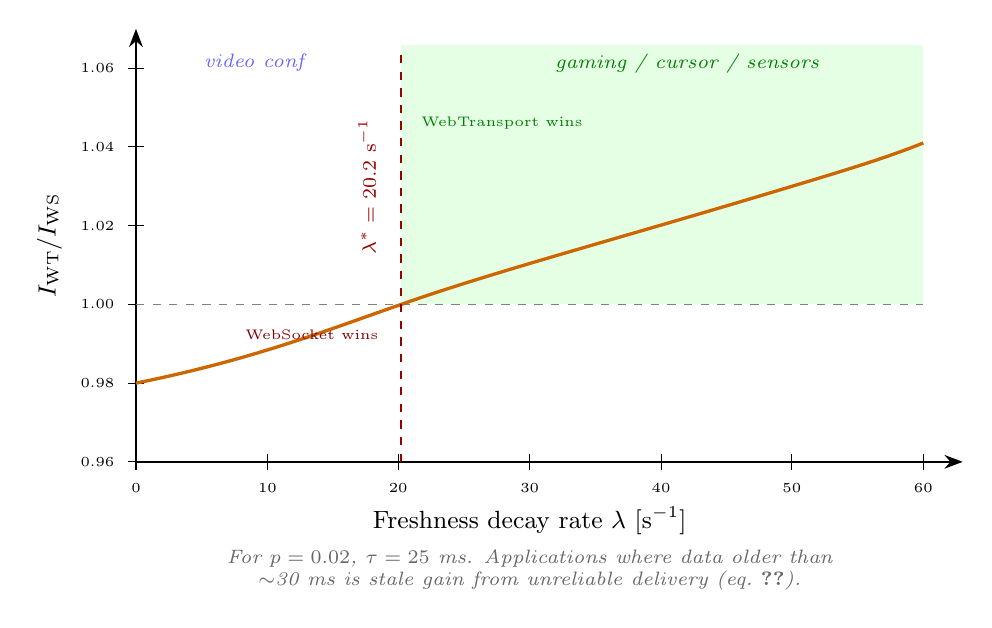
\begin{tikzpicture}[>=Stealth]

% --- Axes ---
\draw[->, thick] (0, 0) -- (10.5, 0);
\draw[->, thick] (0, 0) -- (0, 5.5);

% --- Axis titles (positioned to clear tick labels) ---
\node[font=\small] at (5, -0.75)
  {Freshness decay rate $\lambda$ [s$^{-1}$]};
\node[font=\small, rotate=90] at (-1.1, 2.75)
  {$I_{\text{WT}} / I_{\text{WS}}$};

% --- X-axis labels ---
\foreach \x/\lab in {0/0, 1.67/10, 3.33/20, 5.0/30, 6.67/40, 8.33/50, 10/60} {
  \draw (\x, -0.1) -- (\x, 0.1);
  \node[font=\tiny, anchor=north] at (\x, -0.15) {\lab};
}

% --- Y-axis labels (0.96 to 1.06, each 0.02 = 1 unit) ---
\foreach \y/\lab in {0/0.96, 1/0.98, 2/1.00, 3/1.02, 4/1.04, 5/1.06} {
  \draw (-0.1, \y) -- (0.1, \y);
  \node[font=\tiny, anchor=east] at (-0.15, \y) {\lab};
}

% --- Ratio = 1.0 line (y=2 maps to ratio 1.0) ---
\draw[thin, gray, dashed] (0, 2) -- (10, 2);

% --- Shade WebTransport advantage region ---
% lambda* = 20.2 -> x = 3.37
\fill[green!10] (3.37, 2) rectangle (10, 5.3);

% --- I_WT/I_WS curve: 0.98*exp(lambda*0.001) ---
% Y range: 0.96-1.06 (each 0.02 = 1 unit). lambda=0: y=1, lambda*=20.2: y=2, lambda=60: y=4.05
\draw[very thick, orange!80!black]
  (0, 1.0) .. controls (1.5, 1.3) and (2.5, 1.7) ..
  (3.37, 2.0) .. controls (4.5, 2.4) and (6, 2.8) ..
  (8, 3.4) .. controls (9, 3.7) and (9.5, 3.85) ..
  (10, 4.05);

% --- Threshold line ---
\draw[thick, dashed, red!60!black] (3.37, 0) -- (3.37, 5.2);
\node[font=\scriptsize, red!60!black, anchor=south, rotate=90] at (3.17, 3.5)
  {$\lambda^* = 20.2$ s$^{-1}$};

% --- Application regime labels ---
\node[font=\scriptsize\itshape, text=blue!60, anchor=north] at (1.5, 5.3)
  {video conf};
\node[font=\scriptsize\itshape, text=green!50!black, anchor=north] at (7.0, 5.3)
  {gaming / cursor / sensors};

% --- Mark advantage/disadvantage ---
\node[font=\tiny, text=red!50!black, anchor=north east] at (3.2, 1.8)
  {WebSocket wins};
\node[font=\tiny, text=green!50!black, anchor=north west] at (3.5, 4.5)
  {WebTransport wins};

% --- Annotation ---
\node[font=\scriptsize\itshape, text=black!60, align=center,
  anchor=north] at (5.0, -1.0)
  {For $p = 0.02$, $\tau = 25$~ms. Applications where data older than\\
   ${\sim}$30~ms is stale gain from unreliable delivery (eq.~\ref{eq:wt-advantage}).};

\end{tikzpicture}
\caption{Freshness-weighted information rate ratio $I_{\text{WT}} / I_{\text{WS}}$
  as a function of decay rate $\lambda$. Above the threshold $\lambda^*$,
  WebTransport's unreliable datagrams deliver more useful information per
  unit time than WebSocket's reliable delivery, because retransmission
  wastes capacity on stale data.}
\label{fig:freshness}
\end{figure}

\subsection{Projections Summary and Practical Implications}

\begin{table}[ht]
\centering
\small
\renewcommand{\arraystretch}{1.4}
\begin{tabularx}{\textwidth}{lXXX}
\toprule
\textbf{Measure} & \textbf{March 2026} & \textbf{2027--2028} &
  \textbf{2029--2031} \\
\midrule
Channel capacity $C_{\text{link}}$ &
  120~Mbps &
  150~Mbps &
  250~Mbps \\
HOL blocking factor $(1\!-\!p)^{n-2}$ at $n\!=\!8$ &
  0.94 ($p\!=\!0.01$) &
  0.94 &
  0.97 ($p\!=\!0.005$) \\
Source coding gap $\Delta$ &
  VP9: $\sim$0.8 &
  AV1 HW: $\sim$0.5 &
  AV1 opt: $\sim$0.4 \\
$I_{\text{net}}$ per 720p stream &
  1.3--2.2~Mbps &
  0.9--1.6~Mbps &
  0.6--1.1~Mbps \\
Max 720p streams in $C_{\text{link}}$ &
  $\sim$55--90 &
  $\sim$95--165 &
  $\sim$230--415 \\
E2EE availability &
  Chrome only &
  Cross-browser &
  SFrame $n$-party \\
WebTransport coverage &
  82\% &
  $\sim$100\% &
  100\% \\
Freshness threshold $\lambda^*$ &
  20.2~s$^{-1}$ &
  $\sim$18~s$^{-1}$ &
  $\sim$15~s$^{-1}$ \\
\bottomrule
\end{tabularx}
\caption{Information-theoretic measures across time horizons. $\Delta$
  is the coding efficiency gap (\ref{eq:coding-gap}), $I_{\text{net}}$
  is the net information rate (\ref{eq:inet}), and $\lambda^*$ is the
  freshness decay threshold above which WebTransport dominates WebSocket
  (\ref{eq:wt-advantage}).}
\label{tab:projections}
\end{table}

The trajectory is clear: the combination of improving source coding
(AV1 hardware), expanding channel capacity (broadband growth), and
maturing transport protocols (QUIC universal, WebTransport universal)
drives the \emph{information cost per unit of communicated experience}
steadily downward. The remaining question is not whether the
Shannon capacity suffices --- it already does, by orders of magnitude
--- but how efficiently the protocol stack converts that capacity into
delivered, fresh, secure information at the application layer. By
2030, the gap between theoretical capacity and realized throughput will
be the narrowest it has ever been for browser-based real-time
communication.

\subsubsection{What the Theory Means for Applications}

The equations and figures in this appendix are not purely academic. Each
theoretical result maps to a concrete design decision that application
developers face today and over the next five years.

\textbf{Codec selection determines bandwidth cost, not quality.}
The rate-distortion analysis (Section~A.2, Figure~\ref{fig:rate-distortion})
shows that AV1 operates at roughly 46\% of H.264's bit rate for equivalent
perceptual quality at 720p. In practice, this means a WebRTC application
switching from H.264 to AV1 can either halve its bandwidth consumption at
the same quality or substantially increase resolution (e.g., 720p to 1080p)
within the same bandwidth envelope. By 2030, with AV1 hardware encoding
ubiquitous and the coding gap $\Delta$ approaching 0.4, further codec
improvements yield diminishing returns --- the stack will be operating close
enough to the Shannon rate-distortion bound that the next generation of
efficiency gains will come from transport and architecture, not codecs alone.

\textbf{QUIC's advantage is situational but decisive on bad networks.}
The head-of-line blocking analysis (Section~A.1.1,
Figure~\ref{fig:hol-blocking}) shows that QUIC's per-stream throughput
advantage over TCP is modest on good networks (6\% at 1\% loss) but
substantial on degraded ones (34\% at 5\% loss). The practical implication
is that applications targeting mobile users, emerging markets, or congested
enterprise networks --- precisely the environments where real-time
communication is hardest --- benefit disproportionately from QUIC-based
transports. For a video conference with 8 participants on a cellular
connection experiencing 3--5\% packet loss, the difference between QUIC and
TCP is the difference between usable and degraded video.

\textbf{Connection latency is a solved problem for returning users.}
The handshake analysis (Section~A.1.2) shows that QUIC 0-RTT eliminates
connection establishment overhead entirely for resumed connections. For a
WebTransport application that a user opens daily --- a collaboration tool,
a live dashboard, a recurring meeting client --- the time to first useful
byte drops to zero. The 1.125~MB of wasted capacity during a TCP+TLS
handshake on a 120~Mbps link may seem small, but for latency-sensitive
applications where the first 100~ms of perceived responsiveness determines
user experience, the difference is measurable.

\textbf{Bandwidth surplus enables architectural ambition.}
The effective information rate analysis (Section~A.3,
Figure~\ref{fig:inet-capacity}) reveals the most consequential practical
finding: a single 720p video stream consumes a vanishing fraction of
available link capacity (under 0.5\% by 2030). This surplus is not merely
``headroom'' --- it is the resource that makes new application architectures
feasible. A 250~Mbps link can theoretically carry 230--415 simultaneous 720p
streams. In practice, this means applications can afford to run multiple
concurrent media flows (video, screen share, spatial audio), data channels
(collaborative editing, file transfer), and telemetry streams without
contending for bandwidth. The constraint shifts from ``can the network carry
this?''\ to ``can the application manage this complexity?''

\textbf{End-to-end encryption adds negligible overhead.}
The security analysis (Section~A.4) confirms that the nested DTLS-SRTP plus
E2EE architecture imposes no meaningful information-theoretic cost. The key
entropy ($2^{128}$) exceeds the information content of any practical session
by a factor of at least 3. For application developers, this means E2EE can
be treated as a default rather than a premium feature --- there is no
bandwidth, latency, or capacity penalty for encrypting at the application
layer on top of the transport-layer encryption that WebRTC already mandates.
The only constraint is API availability, which moves from Chrome-only (2026)
to universal (2028).

\textbf{WebTransport unlocks real-time data that WebSocket cannot serve.}
The freshness analysis (Section~A.5, Figure~\ref{fig:freshness}) quantifies
when unreliable delivery outperforms reliable delivery: any data with a
useful half-life below approximately 34~ms benefits from WebTransport's
unreliable datagrams. This covers a wide class of interactive applications
--- game state synchronization, live cursor and pointer sharing, real-time
sensor feeds, collaborative whiteboard strokes --- where retransmitting a
stale update is worse than dropping it. Before WebTransport, these
applications had to choose between WebSocket (reliable but stale under loss)
and WebRTC DataChannel (unreliable mode available but requiring the full
peer-to-peer ICE/DTLS machinery). WebTransport provides the unreliable
mode with a simple client-server model over HTTP/3, removing the
architectural overhead.

\textbf{The overall picture: the stack converges on efficiency.}
Taken together, the information-theoretic measures trace a consistent
trajectory. The protocol stack is converging toward the theoretical limits
established by Shannon: codecs approach the rate-distortion bound, transports
eliminate unnecessary blocking and handshake overhead, and encryption adds
negligible cost. By 2030, the practical distance between what the standards
deliver and what information theory permits will be the smallest it has ever
been for browser-based real-time communication. The consequence for
application developers is that the infrastructure --- standards, hardware,
and networks --- will no longer be the binding constraint. The remaining
challenge is purely architectural: how to compose these efficient, universal
primitives into applications that fully exploit the capacity and low latency
they provide.


\end{document}
